\documentclass[10pt,twocolumn]{article}
\usepackage[a4paper,margin=15mm]{geometry}
\usepackage{amsmath,amssymb}
\usepackage{amsthm}
\theoremstyle{definition}
\newtheorem{theorem}{Theorem}
\newtheorem{proposition}{Proposition}
\newtheorem{corollary}{Corollary}
\newtheorem{remark}{Remark}
\newtheorem{example}{Example}
\newtheorem{definition}{Definition}
\newtheorem{openproblem}{Open Problem}
\usepackage{graphicx}
\usepackage{booktabs,array,calc}
\usepackage[font=small,labelfont=bf]{caption}
\usepackage[colorlinks=true]{hyperref}
\usepackage{etoolbox}
\providecommand{\tightlist}{\setlength{\itemsep}{0pt}\setlength{\parskip}{0pt}}
\setcounter{secnumdepth}{-1}
\emergencystretch=3em
\allowdisplaybreaks
\AtBeginDocument{%
  \BeforeBeginEnvironment{equation}{\small}%
  \BeforeBeginEnvironment{equation*}{\small}%
  \BeforeBeginEnvironment{align}{\small}%
  \BeforeBeginEnvironment{align*}{\small}%
  \BeforeBeginEnvironment{gather}{\small}%
  \BeforeBeginEnvironment{gather*}{\small}%
  \BeforeBeginEnvironment{multline}{\small}%
  \BeforeBeginEnvironment{multline*}{\small}%
  \BeforeBeginEnvironment{flalign}{\small}%
  \BeforeBeginEnvironment{flalign*}{\small}%
}

\begin{document}
\title{An Obstruction Calculus for Viability under Incomplete Observation}
\author{Amin Abaee\\[0.35em]
{\small Independent Researcher}\\[0.55em]
{\small\href{https://orcid.org/0000-0002-0019-1842}{ORCID: 0000-0002-0019-1842}}\\[0.3em]
{\small\href{mailto:amin\_abaee@ut.ac.ir}{amin\_abaee@ut.ac.ir}}}
\date{September 10, 2026}
\maketitle

\begin{abstract}

Under perfect measurement the viability kernel --- the set of states
from which some feedback keeps the system within its constraints --- is
characterized by tangency conditions. Under incomplete observation the
sufficiency direction has a canonical answer in Veliov's
output-feedback regulation condition and the estimation-tube reduction.
The complementary direction --- certifying that no observation-based
policy is viable --- has received less systematic treatment.

This paper develops that instrument: a calculus of obstruction
certificates, sound sufficient conditions for nonviability (equivalently, necessary conditions for viability), finitely
checkable in the finite-state, polyhedral, and finite-horizon cases and analytic drift-and-timing conditions elsewhere. They do not exhaust the complement of the epistemic kernel, the kernel's observation-based counterpart; in finite systems backward recursion is complete. Five mechanisms are established --- two finitely checkable, two
closed-form conditional, one minimal --- with a sixth under a
policy-class restriction. The central common-action obstruction shows
that when the safe controls of compatible states intersect emptily, no
observation-based policy is viable, though every compatible state is
individually viable under full information. The others are a finite-time
exit certificate under an Isaacs-type drift condition, an
epistemic-emptiness construction in which a constant observation merges
states with incompatible admissible controls, a delayed-information
obstruction with an explicit timing bound, and a certification limit:
an exact observation-only certifier exists iff safe-set
membership is constant on the observation fibres. The sixth, a
certainty-equivalence trap, empties the kernel of the uncorrected controller under a biased
observation even when the perfect-information kernel is nonempty.

The calculus is positioned against barrier certificates and estimation
tubes, and its monitoring and institutional consequences ---
observation timing, coarseness, aggregation, and bias --- are drawn.

\end{abstract}

\textbf{Keywords:} viability theory; viability kernel; obstruction
certificates; robust viability; epistemic viability; output feedback;
sustainability governance; information structures; partial observation

\textbf{Mathematics Subject Classification:} 49J53; 93B03; 93C41; 91B76

\subsection{1. Introduction}\label{introduction}

\subsubsection{1.1 The problem}\label{the-problem}

Viability theory characterizes the states of a constrained control system from which at least one control can keep every future state within a constraint set (Aubin, 1991). For sustainability problems the constraints are floors --- stock levels, service thresholds, safety margins --- and viability is the formal counterpart of maintaining a development path rather than merely optimizing it (B\'en\'e, Doyen, and Gabay, 2001; De Lara and Doyen, 2008;
Doyen et al., 2012; Doyen and Gajardo, 2020). The theory under
\emph{perfect measurement} is complete in the relevant sense: the
viability kernel exists as the largest viable subset, and Nagumo-type
tangency conditions certify it.

Sustainability governance, however, operates under \emph{incomplete
observation}. Stocks are assessed at discrete review intervals.
Indicators are coarser than the state. Some stocks are unobserved
altogether. And the information that does arrive may arrive late. This paper addresses that side: for an incomplete observation structure, it develops instruments that certify that no observation-based policy is viable --- that the infeasibility is due to the information structure, not to the dynamics.

Floors in sustainability assessment are typically constraints on the
productive base --- the state of the system that yields the measured
output --- rather than on the output itself. Such a base can be read as
natural capital, as a stock, or as a slowly regenerating flow of
services; these are overlapping readings of the same asset rather than
mutually exclusive ones, and what makes a use of it sustainable is
whether the use falls on the yield or on the base itself. Across
assets, whether the base behaves as a flow or as a stock is a
continuum, set by its regeneration timescale relative to the rate of
use --- a continuum that runs from a season, through a year, to
geological time for a mineral deposit. If a base regenerates too
slowly for the rate at which it is taken, drawdown is still
liquidation.

A base can also erode while measured output is maintained: the
degradation is not yet reflected in the measured quantity, or it is
offset by a higher per-unit service, because use may draw on the base
rather than on its yield. The signal that would reveal the erosion is
accordingly often the one that is coarse, postponed, or absent.
Incomplete observation is therefore structural to the certification
problem, not merely a practical limitation; the sufficiency literature
and the obstruction calculus of this paper address the same underlying
indeterminacy rather than competing ones.

The question splits naturally. The sufficiency direction has a canonical literature: Veliov (1993) gives conditions for the existence of an output-feedback regulation map under incomplete and inexact measurement, reducing under perfect measurement to the classical viability condition (Haddad, 1981); the estimation-tube programme (Cardaliaguet, Quincampoix, and Saint-Pierre, 2007) absorbs imperfect information into an estimation space of sets of compatible states with no loss of value; and barrier certificates certify safety (Prajna and Jadbabaie, 2004; Prajna, Jadbabaie, and Pappas, 2007), with converse and hybrid necessary-and-sufficient characterizations (Prajna and Rantzer, 2005; Maghenem and Sanfelice, 2019). What that literature does not supply is the necessity side: a calculus of obstruction certificates. An obstruction certificate is a checkable witness that no observation-based policy exists --- finite in the finite-state and polyhedral cases --- and the argument it makes is that a prescribed class of observation-based policies fails not because a particular policy is bad, but because the information structure leaves no room for any policy. In the polyhedral common-action and certification forms (Theorem~\ref{thm:common-action} and Proposition~\ref{prop:fibre}) it is a finite, checkable test; the drift certificates of Theorem~\ref{thm:exit} and Theorem~\ref{thm:delayed} are not finite objects, one exhibiting an enforcement selection and the other bounding the timing uniformly over every policy. Veliov's condition tells us when output feedback can work; the obstruction calculus tells us when it cannot, and for the borderline cases it identifies which quantitative feature of the observation design --- timing, coarseness, bias, aggregation --- is responsible.

\subsubsection{1.2 Contributions}\label{contributions}

Five obstruction mechanisms are developed, each with a complete proof,
and a sixth is exhibited under a policy-class restriction:

\begin{enumerate}
\def\labelenumi{\arabic{enumi}.}
\item
  \textbf{The finite-time exit certificate} \emph{(closed-form conditional)} (Theorem~\ref{thm:exit}). Under a
  Dini-drift condition of Isaacs type --- the disturbance chooses after
  the control --- the disturbance can force exit from the safe set
  within an explicit time bound, for \emph{every} admissible control of
  any information structure. This is the base obstruction: when it
  applies, the viability question is closed without any
  observation-theoretic argument.
\item
  \textbf{Epistemic emptiness by admissibility} \emph{(minimal construction)} (Proposition~\ref{prop:emptiness}, a minimal
  construction). A constant observation merges states whose
  \emph{admissible} controls differ: the state-dependent control set
  forces a single common action, and that action is unsafe at the
  boundary, so the unresolved initial observation fibre lies outside the
  epistemic kernel, even though every physical state is viable under
  full information. The mechanism is admissibility --- the common-action
  obstruction of Theorem~\ref{thm:common-action} at minimal size --- and Example~\ref{ex:hidden-mode} gives the hidden-mode instance.
\item
  \textbf{The instantaneous common-action obstruction} \emph{(finitely checkable)} (Theorem~\ref{thm:common-action},
  Example~\ref{ex:hidden-mode}). If the safe-control sets of the states compatible with the
  current information set intersect emptily, then no observation-based
  policy is viable, even though every compatible state is individually
  viable under full information. The failure is purely informational: no
  stochasticity, no estimation error.
\item
  \textbf{The delayed-information obstruction} \emph{(closed-form conditional)} (Theorem~\ref{thm:delayed}). If the
  information needed to distinguish safe from unsafe compatible states
  arrives only at time \(T_{\mathrm{obs}}\), and the disturbance can
  force constraint violation earlier than \(T_{\mathrm{obs}}\), then no
  observation-based policy is viable. The timing bound
  \(\inf q / \varepsilon < T_{\mathrm{obs}}\) is stated explicitly:
  information may be accurate but arrive too late.
\item
  \textbf{The fibre certification criterion} \emph{(finitely checkable)} (Proposition~\ref{prop:fibre}, Corollary~\ref{cor:certainly-safe}).
  An exact observation-only safety certifier --- a function of the
  observation that returns ``safe'' exactly on the safe set --- exists
  if and only if safe-set membership is constant on every observation
  fibre. The certainly-safe set is the sound relaxation: the largest set
  of observations that can be labeled safe without further information.
\item
  \textbf{The certainty-equivalence trap} \emph{(policy-class restriction)} (Remark~\ref{rem:ce-trap}). Even an
  \emph{injective} observation empties the kernel of a system whose
  perfect-information kernel is nonempty for the canonical
  certainty-equivalence controller --- the perfect-information zeroing
  law applied to the uncorrected observation. The trap is a
  policy-specific failure: a controller that uses the observation map's
  structure (the bias correction) restores viability.
\end{enumerate}

The calculus is organized by a single selector principle (Proposition~\ref{prop:selector}, Section 2.4):
observation-based viability is the existence of one response ---
admissible, safe, and recursively viable --- for every compatible state,
and each certificate proves that a specific response correspondence is
empty; the obstructions are nested in a ladder
(Proposition~\ref{prop:ladder}). Five refinements complete the picture:
a comparison-function form sharpens the exit-time bound
(Remark~\ref{rem:comparison}); a uniform-margin condition connects the
instantaneous and tube obstructions
(Proposition~\ref{prop:uniform-margin}); the timing obstruction has a
sharp threshold form (Remark~\ref{rem:sigma}); a Helly-type sparse
witness bounds the common-action obstruction by \(m+1\) compatible
states (Proposition~\ref{prop:helly}); and backward belief recursion is
sound and complete on any finite horizon in finite systems
(Theorem~\ref{thm:finite-horizon}). The epistemic kernel is monotone in
action sets, disturbances, information, and policy class
(Proposition~\ref{prop:monotone}).

Throughout, ``obstruction'' means a \emph{certified} failure. Theorem~\ref{thm:exit} and Theorem~\ref{thm:delayed} each exhibit the violating constraint, an admissible disturbance,
and the quantitative bound that make failure inevitable, for every policy in the prescribed class; Proposition~\ref{prop:emptiness} and Theorem~\ref{thm:common-action} exhibit the incompatible
admissible controls --- the merged observation whose incompatible safe
controls certify emptiness --- with no quantitative bound claimed there;
and Proposition~\ref{prop:fibre} is the converse-side characterization of the certification
limit itself. The calculus is positioned against
the barrier-certificate literature (Section 6.2) and the estimation-tube
programme (Section 6.3), and its consequences for the design of
monitoring and indicators in sustainability governance are drawn in
Section 6.4.

\subsubsection{1.3 Related work}\label{related-work}

The viability-theory background is Aubin (1991), Aubin, Bayen, and Saint-Pierre (2011), and the kernel approximation theory of Saint-Pierre (1994); robust viability is Aubin and Frankowska (1990) and Frankowska (1989). Under incomplete measurement, the sufficiency theorem is Veliov (1993), viability with a priori unknown but observable parameters is Quincampoix and Veliov (1994), and the estimation-set reduction is Cardaliaguet, Quincampoix, and Saint-Pierre (2007). On the failure side, Aubin (2001) characterizes the complement of the kernel --- Poincar\'e's ``shadow'' --- together with the capture basins, and Aubin and Catt\'e (2002) supply the bilateral-fixed-point and discriminating-kernel calculus; the certificates of Section 3 are one-sided, observation-constrained analogues of that programme. In verification, barrier certificates originate with Prajna and Jadbabaie (2004), with worst-case and converse results in Prajna, Jadbabaie, and Pappas (2007) and Prajna and Rantzer (2005) and hybrid characterizations in Maghenem and Sanfelice (2019). The sustainability application domain is B\'en\'e, Doyen, and Gabay (2001), De Lara and Doyen (2008), Doyen et al. (2012), and Doyen and Gajardo (2020). To our knowledge, the obstruction certificates of Theorem~\ref{thm:common-action}, Theorem~\ref{thm:delayed}, and Proposition~\ref{prop:fibre} --- in particular the certification criterion and the timing bound --- have not been stated in this form; the elementary facts on which they rest (quantifier commutation and Dini comparison) are classical.

\subsubsection{1.4 Organization}\label{organization}

Section 2 fixes the framework: the control system, the viability kernel
hierarchy, observation structures, information states, the safe-control
correspondence, and the selector principle (Proposition~\ref{prop:selector}). Section 3 develops the obstruction calculus (Theorem~\ref{thm:finite-horizon}--\ref{thm:exit}, Propositions~\ref{prop:uniform-margin}--\ref{prop:emptiness}, Remarks~\ref{rem:sigma}--\ref{rem:comparison}, and Example~\ref{ex:hidden-mode}): finite-horizon completeness, the instantaneous common-action obstruction with its ladder and sparse witness, the delayed-information obstruction with its threshold form, and --- as supporting certificates --- the finite-time exit certificate and the admissibility obstruction. Section 4 develops the certification limits
(Proposition~\ref{prop:fibre}, Corollary~\ref{cor:certainly-safe}, Remark~\ref{rem:ce-trap}). Section 5 reviews the sufficiency landscape, cited rather than re-derived. Section
6 discusses the position of the calculus relative to barrier
certificates and estimation tubes, states the monotonicity of the
epistemic kernel (Proposition~\ref{prop:monotone}), and draws the governance
consequences. Sections 7--9 develop the new material: complete characterizations and the residual gap (Section 7), a calibrated case study with a coverage audit (Section 8), and the probabilistic belief-state development (Section 9). Section 10 concludes. Proof sketches of the Section 3 results are given in the main text; the complete proofs, the expanded sufficiency review, and the auxiliary constructions are collected in the Supplementary Material.



\subsection{2. Framework}\label{framework}

\subsubsection{2.1 The control system and the kernel
hierarchy}\label{the-control-system-and-the-kernel-hierarchy}

This section fixes the mathematical objects used throughout the paper:
the control system, the disturbance structure, the constraint set, and
the four kernels (perfect-information, robust, epistemic, and
institutionally restricted) that organize the analysis.

Fix a state space \(X \subseteq \mathbb{R}^n\), a control set \(U\), a
disturbance set \(D\), and dynamics
\[\dot x(t) = f(x(t), u(t), d(t)), \qquad u(t) \in U(x(t)), \quad d(t) \in D(x(t)),\]
with \(f\) continuous, \(U\) and \(D\) set-valued with closed graph and
nonempty compact values, and admissible controls and disturbances taken
to be measurable selections --- the standing solution-existence conditions:
every selection pair admits a Carath\'eodory solution, and the
convexified relaxed inclusion of Section 3.5 satisfies the Marchaud
conditions of the viability literature (Aubin, 1991). Let \(\mathcal{V} \subseteq X\) be a closed
constraint set. A \emph{causal policy} \(\pi\) is a map from the
observation record to controls, respecting the specified information structure. The standard objects are:

\begin{itemize}
\tightlist
\item
  \(\mathrm{Viab}(\mathcal{V}; U, \pi_{\mathrm{perf}})\): the
  \textbf{viability kernel} under full-information (state-feedback)
  policies --- the largest closed subset of \(\mathcal{V}\) from which
  there exists a state-feedback control keeping the trajectory in
  \(\mathcal{V}\) for all time --- no disturbance, or a known
  disturbance trajectory (Aubin, 1991).
\item
  \(\mathrm{RViab}(\mathcal{V})\): the \textbf{robust kernel}, the
  largest subset of \(\mathcal{V}\) from which there exists a
  state-feedback policy keeping every trajectory --- for \emph{every}
  admissible disturbance realization --- in \(\mathcal{V}\) (Aubin and
  Frankowska, 1990).
\item
  \(\mathrm{ERViab}_{\mathcal{I}}(\mathcal{V})\): the \textbf{robust
  epistemic kernel} --- the object of this paper (Definition~\ref{def:kernel}). Its
  elements are \emph{states of information}, not physical states
  (Section 2.3). The non-robust counterpart
  \(\mathrm{EViab}_{\mathcal{I}}(\mathcal{V})\) is the non-robust contrast class (Section 2.3).
\end{itemize}

Projected to physical state space --- with
\(\mathrm{proj}_{\exists}(\mathfrak{B}) = \bigcup_{B \in \mathfrak{B}} B\)
the \emph{existential} projection of a collection \(\mathfrak{B}\) of
information states, applied to the first two terms, whose elements are information states --- the informational hierarchy
reads
\[
\begin{aligned}
\mathrm{proj}_{\exists}\big(\mathrm{IRViab}_{\mathcal{J}}(\mathcal{V})\big)&\;\subseteq\; \mathrm{proj}_{\exists}\big(\mathrm{ERViab}_{\mathcal{I}}(\mathcal{V})\big) \\
&\;\subseteq\; \mathrm{RViab}(\mathcal{V}) \;\subseteq\; \mathrm{Viab}(\mathcal{V}),
\end{aligned}
\]
where \(\mathrm{IRViab}_{\mathcal{J}}(\mathcal{V})\) is the institutionally restricted kernel of Section 6.4. The physical implication of epistemic viability is the
inclusion at the level of beliefs:
\(B_0 \in \mathrm{ERViab}_{\mathcal{I}}(\mathcal{V}) \Rightarrow B_0 \subseteq \mathrm{RViab}(\mathcal{V})\).
Each inclusion can be strict, with a distinct cause: robust contraction
arises from disturbances; epistemic contraction from
indistinguishability; institutional contraction from restricted
authority, enforcement, and allocation. The present paper characterizes
the \emph{epistemic} contraction: the mechanisms by which
indistinguishability empties or shrinks the kernel.

\subsubsection{2.2 The safe-control
correspondence}\label{the-safe-control-correspondence}

For a constraint set \(\mathcal{V}\) described by finitely many \(C^1\)
constraint functions,
\(\mathcal{V} = \{ x : q_j(x) \ge 0,\ j = 1..m \}\), define the
\textbf{safe-control correspondence} at \(x \in \mathcal{V}\):
\[
\begin{aligned}
\mathcal{R}_{\mathcal{V}}(x) \;=\; \bigl\{ u \in U(x) : {}& \forall d \in D(x),\; \forall j \text{ with } q_j(x) = 0,\\
& \nabla q_j(x) \cdot f(x, u, d) \ge 0 \bigr\},
\end{aligned}
\]
the set of controls whose drift is inward (subtangential) on every
active constraint face, uniformly over the disturbance. For \(x\) in the
interior of \(\mathcal{V}\) (no active constraints),
\(\mathcal{R}_{\mathcal{V}}(x) = U(x)\). Two levels of the tangency condition are distinguished throughout. (i) \emph{Local reading.} The correspondence is applied to the constraint set itself: by Nagumo's theorem (Nagumo, 1942) in its robust form, if \(\mathcal{V}\) is closed and
\(\mathcal{R}_{\mathcal{V}}(x) \neq \varnothing\) on
\(\partial\mathcal{V}\) with a measurable selection
\(u(x) \in \mathcal{R}_{\mathcal{V}}(x)\), then \(\mathcal{V}\) is
itself robustly invariant,
i.e.~\(\mathrm{RViab}(\mathcal{V}) = \mathcal{V}\) (Aubin, 1991;
Frankowska, 1989). (ii) \emph{Kernel reading.} When \(\mathcal{V}\) is not invariant, viability of a point \(x_0 \in \mathcal{V}\) requires instead a selection \(u(x) \in \mathcal{R}_G(x)\) along the trajectory, where \(G = \mathrm{RViab}(\mathcal{V})\) and \(\mathcal{R}_G\) is the same correspondence computed on the kernel: points of
\(\mathcal{V} \setminus G\) may admit controls that are instantaneously
safe while every trajectory must exit later. The obstruction
theorems below are \emph{local certificates against
\(\mathcal{R}_{\mathcal{V}}\)}: exhibiting a state at which even the
weaker pointwise condition fails certifies exclusion from the kernel,
and this is the reading in which the certificates are used. The
correspondence is the bridge between the pointwise (tangency) and the
global (kernel) description, and it is the object the observation
structure acts upon: an observation-based policy can select controls
only as a function of the observation record.

\subsubsection{2.3 Observation structures, information states, and
epistemic
kernels}\label{observation-structures-information-states-and-epistemic-kernels}

\textbf{Conventions.} Throughout, the plant evolves in continuous time
and a policy acts at review times, holding the selected action until the
next review; the observation record is generated by the observation map
\(O\) (the error, hidden-parameter, and delay extensions are noted
below). Between reviews the record \(y(t)=O(x(t))\) is observed
continuously but cannot change the held action; the certificates of
Sections 3.2--3.3 and 3.6 use the record only through what it discriminates
(observation-equivalence), so they remain valid under any refinement of
the within-interval record that does not separate compatible branches.
A policy is observation-based if its action depends on the
record only through the information set \(B_t\); under the delay-free
set-membership semantics used here the information set is a sufficient
statistic, so observation-based and record-based policies coincide (with
delays, hidden parameters, or history-dependent constraints the belief
must be augmented and sufficiency is not automatic; Section 6.5). The disturbance
is chosen adversarially after the control (the Isaacs order of
Theorems~\ref{thm:exit} and \ref{thm:common-action}), an action outside
\(U(x)\) at a compatible state \(x\) is itself a failure (Section 2.4),
and constraint violation is the strict inequality \(q<0\).

An \textbf{observation structure} \(\mathcal{I} = (Y, O)\) is a
measurable space \(Y\) and an observation map \(O : X \to Y\). The
policy observes \(y(t) = O(x(t))\). At time \(t\), the
\textbf{information set} (belief) of a regulator who knows the dynamics,
the disturbance class, its own applied controls \((u(s))_{s<t}\), and the record \((y(s))_{s \le t}\) is
\[
\begin{aligned}
B_t \;=\; \bigl\{ \xi(t) : {}& \xi(0) \in B_0,\\
& \dot\xi(s) = f(\xi(s), u(s), d(s)),\ d(s) \in D(\xi(s)),\\
& O(\xi(s)) = y(s) \text{ for all observed } s \le t \bigr\},
\end{aligned}
\]
where the applied control history \(u(\cdot)\) in the dynamics is
the regulator's own --- common to every candidate trajectory --- and
\(\xi(\cdot)\) ranges over candidate trajectories: the set of current
states compatible with the record and the applied controls. We assume the standard set-membership semantics (Kurzhanski and V\'alyi, 1997), so that \(B_t\) contains every state
consistent with the observations and the applied controls. (With
observation error, the equality becomes membership
\(y(s) \in H(\xi(s), v(s))\); with hidden parameters the belief lives in
\(X \times \Theta\); with delays it lives in a history space --- the extensions are noted as open in Section 6.5.) A policy is
\textbf{observation-based} if \(u(t)\) depends on the record only
through \(B_t\); this is a special case of record-based policies, and
the two coincide when the belief is a sufficient statistic for the
decision problem, which holds in the delay-free set-membership semantics used
throughout. We write \(U^B(B) = \bigcap_{x \in B} U(x)\) for the
controls available at every compatible state --- the only controls an
observation-based policy may select without risking inadmissibility.

\begin{definition}[robust epistemic kernel]\label{def:kernel}

\(B_0 \in \mathrm{ERViab}_{\mathcal{I}}(\mathcal{V})\) if there exists a
nonanticipative observation-based policy \(\pi\) such that, for every
compatible initial state \(x_0 \in B_0\) and every admissible
disturbance realization \(d(\cdot)\), the trajectory of
\(\dot x = f(x, u(t), d(t))\) generated from \(x_0\) by \(\pi\)'s
actions under \(d(\cdot)\) --- the record being the one that
\((\pi, d(\cdot))\) generates --- remains in \(\mathcal{V}\) for all
time. (This is the standard exists-strategy-for-all-realizations form. The quantifier order is essential: the record is generated by the realization, so conditioning the admissible realizations on the record would be circular.) Admissible initial
beliefs are the compact information sets \(B_0 \subseteq X\) generated
by the observation structure --- the observation fibres \(O^{-1}(y)\),
\(y \in O(X)\), in the constructions of Sections 3.2--3.3 and 3.6. The existential (non-robust) counterpart \(\mathrm{EViab}_{\mathcal{I}}(\mathcal{V})\) is the non-robust contrast class.

\end{definition}

We use \(\mathrm{ERViab}\) throughout, since the disturbance classes of sustainability problems are adverse by construction. The theorems are stated for this robust notion; they do not transfer a fortiori to the non-robust contrast class \(\mathrm{EViab}_{\mathcal{I}}(\mathcal{V})\), in which there exist an observation-based policy and \emph{some} admissible disturbance realization under which every compatible trajectory remains in \(\mathcal{V}\) for all time. Since the robust kernel is contained in the non-robust one, an observation-based policy may exist there that no robust policy survives.

The thesis is now precise:
\textbf{the epistemic kernel is the greatest recursively viable collection of information states in the sense of the estimation-space reduction cited in Section 5; common-action compatibility is a necessary one-step condition, but not by itself a
complete characterization --- and the obstruction calculus certifies,
mechanism by mechanism, the information states outside it.}

\subsubsection{2.4 Notation}\label{notation}

We collect the principal symbols used throughout the paper and fix the two structural symbols: the \textbf{observation structure} is always
\(\mathcal{I}\) (calligraphic I) and the \textbf{institution} of Section
6.4 is always \(\mathcal{J}\) (calligraphic J); no other letter serves either role. The state space is \(X \subseteq \mathbb{R}^n\); the
control set is \(U\) (set-valued \(U(x)\) at state \(x\)); the
disturbance set is \(D\) (set-valued \(D(x)\)). The dynamics are
\(\dot x = f(x,u,d)\). The closed constraint set is
\(\mathcal{V} \subseteq X\), described by finitely many \(C^1\)
constraint functions \(q_j\) (\(j = 1,\ldots,m\)). The safe-control
correspondence at \(x \in \mathcal{V}\) is
\(\mathcal{R}_{\mathcal{V}}(x)\). The observation structure is
\(\mathcal{I} = (Y, O)\) with observation map \(O : X \to Y\); the
information set (belief) at time \(t\) is \(B_t\); the initial belief is
\(B_0\) --- admissible initial beliefs are the compact information sets
the observation structure generates, the observation fibres
\(O^{-1}(y)\), \(y \in O(X)\), in the constructions. The common
admissible action set at belief \(B\) is
\(U^B(B) = \bigcap_{x \in B} U(x)\) --- the only controls an
observation-based policy may select without risking inadmissibility,
under the convention, used from Proposition~\ref{prop:emptiness} on, that an action outside
\(U(x)\) at a compatible state is itself failure; the common safe-action
set is
\(\mathcal{R}_{\mathcal{V}}^B(B) = \bigcap_{x \in B} \mathcal{R}_{\mathcal{V}}(x)\).
The tube-safe action set at review length \(\Delta\) is
\(\mathcal{A}_{\mathrm{tube}}(B, \Delta) = \{ a : \mathrm{Reach}_{[0,\Delta]}(B, a) \subseteq \mathcal{V} \}\),
where \(\mathrm{Reach}_{[0,\Delta]}(B, a)\) is the \emph{robust} ---
all-disturbance, all-solution --- reachable set of the system from \(B\) under the
held action \(a\) over \([0,\Delta]\). The first informative observation
time is \(T_{\mathrm{obs}}\): the first time the observation record
discriminates between compatible branches --- before it, the branches of
Theorem~\ref{thm:delayed}'s (H4.1) produce identical records. The adverse-selection
correspondences of the exit certificates are
\(D_{\varepsilon}(x,u) = \{ d \in D(x) : D^+ q(x; f(x,u,d)) \le -\varepsilon \}\)
(Theorem~\ref{thm:exit}) and
\(D_{\eta}(x) = \{ d \in D(x) : \nabla q_j(x) \cdot f(x, a, d) \le -\eta/2 \}\)
(Theorem~\ref{thm:common-action}'s proof, local). The upper
right Dini derivative of \(q\) in direction \(v\) is
\(D^+ q(x; v) = \limsup_{h \downarrow 0} [q(x + hv) - q(x)]/h\); for
\(q\) of class \(C^1\) --- the class assumed in the exit theorems ---
\(D^+ q(x; v) = \nabla q(x) \cdot v\).

The kernels of the hierarchy are
\(\mathrm{Viab}(\mathcal{V}; U, \pi_{\mathrm{perf}})\) (perfect
information), \(\mathrm{RViab}(\mathcal{V})\) (robust), and
\(\mathrm{ERViab}_{\mathcal{I}}(\mathcal{V})\) (the robust epistemic
kernel --- Definition~\ref{def:kernel}, the object of this paper), with
\(\mathrm{proj}_{\exists}(\mathfrak{B}) = \bigcup_{B \in \mathfrak{B}} B\)
the existential projection of a collection \(\mathfrak{B}\) of information states. Consistency check: when the observation \(O\) is injective the record determines the state, so the epistemic and robust kernels agree, \(\mathrm{ERViab}_{\mathcal{I}}(\mathcal{V}) = \mathrm{RViab}(\mathcal{V})\), the informational certificates of Sections 3.2--3.3 and 3.6 reduce to the no-merge case, and only the dynamic obstruction of Section 3.5 can certify exclusion --- the definitions degenerate to classical robust viability exactly when observation is perfect. The non-robust counterpart
\(\mathrm{EViab}_{\mathcal{I}}(\mathcal{V})\) is the non-robust contrast class (Section 2.3). The institutionally restricted kernel is \(\mathrm{IRViab}_{\mathcal{J}}(\mathcal{V})\) (Section 6.4). The policy classes
are \(\pi_{\mathrm{perf}}\) (state feedback), \(\Pi_{\mathrm{output}}\),
\(\Pi_{\mathrm{state}}\), and \(\Pi_{\mathrm{CE}}\) --- the
certainty-equivalence class defined in Remark~\ref{rem:ce-trap}: fixed
perfect-information regulation laws applied uncorrected to the
observation. The policy-specific safety set of Section 4.1 is
\(\mathrm{Safe}^{\Pi}_T\); the certainly-safe set of Corollary~\ref{cor:certainly-safe} is
\(\mathcal{Y}_{\mathrm{safe}}\).

Some letters carry site-local meanings. The strip width \(a\) of
Theorem~\ref{thm:exit}'s \(\mathcal{S}_a\) is not the held action
\(a = \pi(B)\) of Theorem~\ref{thm:common-action}'s proof, nor the
pathway vector \(a \ge 0\) of Section 5(d); \(\lambda\) is the Farkas
multiplier of Theorem~\ref{thm:common-action}'s checkability
certificate and the observer decay rate of Section 5(c); and
\(\alpha\) is the comparison function of Remark~\ref{rem:comparison}
and a multiplier of Section 5(d)'s substitution alternative. The
letter \(K\) denotes the safe set of Section 4's certification
problems, while in Section 5(c) it denotes the kernel
itself, with the buffered set \(K_\zeta\) and eroded kernels
\(K^{-c\zeta}\) of Section 5(c). The observation-error map of
Section 2.3 is \(H(\xi, v)\), whereas the harvest vector of
the Supplementary Material is the lowercase \(h\); and the finite-horizon recursion
set \(\mathcal{W}_N\) of Section 3.1 is calligraphic, distinct from
the Lyapunov function \(W = S_1 + S_2\) of the Supplementary Material.

The four correspondences of this section are one skeleton. An
observation-based regulator selects a single response for an entire
information set --- a held action, a feedback segment, or a
safe/unsafe verdict --- and observation-based viability is the existence
of a response that is simultaneously admissible, safe, and recursively
viable for every compatible state and disturbance history. Each
obstruction certificate of Sections 3 and 4 is a checkable sufficient
condition under which one of these response correspondences is empty:
\(U^B(B)\) (admissibility), \(\mathcal{R}_{\mathcal{V}}^B(B)\)
(instantaneous safety), \(\mathcal{A}_{\mathrm{tube}}(B,\Delta)\)
(review-interval safety), or the recursive predecessor of Section 3.1.
The mechanisms differ in which correspondence fails, and the
obstructions are nested (Proposition~\ref{prop:ladder}). The organizing
claim of the calculus is the following, stated once and used implicitly
by every certificate of Sections 3 and 4.

\begin{proposition}[selector principle]\label{prop:selector}
If \(B\in\mathrm{ERViab}_{\mathcal{I}}(\mathcal{V})\) and \(\pi\) is a
policy witnessing viability on \(B\), then at every review time the
action \(a=\pi(B)\) selected by \(\pi\) is a response that is
(i) \emph{admissible}, \(a\in U^B(B)\); (ii) \emph{safe}, keeping every
compatible trajectory in \(\mathcal{V}\) until the next observation ---
\(\mathrm{Reach}_{[0,\Delta]}(B,a)\subseteq\mathcal{V}\) at review
length \(\Delta\); and (iii) \emph{recursively viable}, in that every
post-observation belief reached at the next review is again in
\(\mathrm{ERViab}_{\mathcal{I}}(\mathcal{V})\) under the continuation
of \(\pi\). A belief is therefore viable only if each of the response
correspondences of this section --- \(U^B(B)\),
\(\mathcal{R}_{\mathcal{V}}^B(B)\), \(\mathcal{A}_{\mathrm{tube}}(B,\Delta)\),
and the recursive predecessor of Section 3.1 --- is nonempty along
every reachable branch; hence a certificate that any one of them is
empty at a reachable belief certifies nonviability. In finite systems
the converse is exact (Theorem~\ref{thm:finite-horizon}); in continuous
time the converse is the backward-recursion completion noted in
Section 6.5.
\end{proposition}



\subsection{3. The Obstruction Calculus}\label{the-obstruction-calculus}

\subsubsection{3.1 Finite-horizon completeness (finite systems)}\label{finite-horizon-completeness}

The certificates of Sections 3.2--3.3 and 3.5--3.6 are sufficient conditions, not a
complete characterization of the epistemic kernel. In the finite setting
the calculus is complete: backward recursion over beliefs --- the set-membership analogue of the belief-state recursion of partially observable Markov processes (Smallwood and Sondik, 1973) --- is sound and complete on any finite horizon, and nonviability is certified by a
finite obstruction tree.

Fix finite state, action, disturbance, and observation spaces \(X\),
\(A\), \(D\), \(Y\), a transition map \(x^+ = F(x,a,d)\), an observation
map \(y = O(x,a,d,x^+)\), a safe set \(\mathcal V\subseteq X\), and
admissible-action sets \(U(x)\subseteq A\). For a belief \(B\subseteq X\),
an action \(a\), and an observation \(y\), the post-belief is
\[
\begin{gathered}
\mathrm{Post}(B,a,y) = \bigl\{ x^+\in X : \exists\, x\in B,\ d\in D(x), \\
x^+ = F(x,a,d),\ y = O(x,a,d,x^+) \bigr\},
\end{gathered}
\]
and \(y\) is possible under \((B,a)\) if \(\mathrm{Post}(B,a,y)\neq\varnothing\).
With \(U^B(B)=\bigcap_{x\in B}U(x)\), define the one-step predecessor of a
collection \(\mathcal C\) of beliefs by
\[
\begin{gathered}
\mathrm{Pre}(\mathcal C) = \bigl\{ B\subseteq\mathcal V : \exists\, a\in U^B(B)\ \text{such that}\\
\mathrm{Post}(B,a,y)\in\mathcal C\ \text{for every possible } y \bigr\},
\end{gathered}
\]
and the finite-horizon kernels by \(\mathcal W_0 = \{B : B\subseteq\mathcal V\}\),
\(\mathcal W_{k+1} = \mathrm{Pre}(\mathcal W_k)\).
The \(N\)-step common safe-action set at a belief \(B\) is
\(\mathcal{A}_N(B) = \bigl\{ a \in U^B(B) : \mathrm{Post}(B,a,y) \in \mathcal W_{N-1} \text{ for every possible } y \bigr\}\),
so that \(B \in \mathcal W_N \iff \mathcal{A}_N(B) \neq \varnothing\). The recursion is exact but of worst-case complexity exponential in
\(|X|\) --- the belief space contains up to \(2^{|X|}\) beliefs --- so
finite-checkability is per belief, not a polynomial-time global procedure.

\begin{theorem}[finite-horizon soundness and completeness]\label{thm:finite-horizon}
An initial belief \(B_0\) admits an observation-based policy that keeps
every compatible trajectory in \(\mathcal V\) for \(N\) steps if and only
if \(B_0\in\mathcal W_N\).
\end{theorem}

\emph{Proof sketch.} Both directions are inductions on the horizon. Necessity: a policy safe for \(N\) steps picks \(a \in U^B(B_0)\), and every possible successor belief is safe for \(N - 1\) steps, so \(B_0 \in \mathrm{Pre}(\mathcal{W}_{N-1})\). Sufficiency: choose the witness action at each step, and every reachable state remains in \(\mathcal{V}\) for \(N\) steps.

If \(B_0\notin\mathcal W_N\), the failure is certified by a finite
\textbf{obstruction tree}: at each node \((B,k)\) with \(k\ge1\), for
every \(a\in U^B(B)\) the adversary can choose a possible observation
\(y\) with \(\mathrm{Post}(B,a,y)\notin\mathcal W_{k-1}\); the branches
are the compatible observation-and-disturbance choices that force
violation within \(N\) steps. This is the exact finite-horizon
counterpart of the sufficient certificates of Sections 3.2--3.3 and 3.5--3.6. The recursion reads \(B_0\) as the belief after the
initial observation has been assimilated, and the tree alternates
regulator and nature turns --- the regulator selects an action, the
adversary a compatible observation --- the standard alternating
structure of partial-information games.

\textbf{A one-step instance.} The discrete one-step abstraction of
Example~\ref{ex:hidden-mode} --- transition \(z^+ = z + \theta u\) on
the grid \(z \in \{-1,0,1\}\), preserving the common-action mechanism
--- is the smallest obstruction tree. With
\(z\in\{-1,0,1\}\), \(\theta\in\{-1,+1\}\), \(u\in\{-1,+1\}\),
transition \(z^+=z+\theta u\), safe set \(\mathcal V=\{z\ge 0\}\), and
observation \(O(z,\theta)=z\), the belief \(B_0=\{(0,-1),(0,+1)\}\) has
\(U^B(B_0)=\{-1,+1\}\). Under \(u=+1\) the branch \(\theta=-1\) reaches
\(z^+=-1\) (observed \(-1\)), so
\(\mathrm{Post}(B_0,+1,-1)=\{(-1,-1)\}\notin\mathcal W_0\); under
\(u=-1\) the branch \(\theta=+1\) reaches \(z^+=-1\). Hence
\(B_0\notin\mathcal W_1\), and the obstruction tree is the root
\((B_0,1)\) with two adversary edges, \(\theta=-1\) and \(\theta=+1\),
each terminating in the violation \(z<0\). This is
Theorem~\ref{thm:common-action} in the finite-horizon language; the tree is drawn in the Supplementary Material (Figure~S2).





\subsubsection{3.2 The instantaneous common-action
obstruction}\label{the-instantaneous-common-action-obstruction}

\begin{theorem}[common-action obstruction]\label{thm:common-action}

Let \(B \subseteq \mathcal{V}\) be an information set of the specified observation structure (the safe-control correspondence
\(\mathcal{R}_{\mathcal{V}}\) is defined on \(\mathcal{V}\), so the
belief is taken inside it). Suppose the following hypotheses hold.

(H3.1) The selected action is held until the next observation (sampled
review: no informative observation arrives before the next action must
be selected, and the policy holds the selected action over the review
interval --- the institutional reading; without a positive dwell time
the instantaneous statement below must be replaced by the tube-safety statement below).

(H3.2) Either the \textbf{common admissible action set} is empty,
\[U^B(B) \;=\; \bigcap_{x \in B} U(x) \;=\; \varnothing, \qquad \text{(admissibility obstruction)}\]
or the \textbf{common safe-action set} is empty while common
admissibility holds,
\begin{gather}
\mathcal{R}_{\mathcal{V}}^B(B) \;:=\; \bigcap_{x \in B} \mathcal{R}_{\mathcal{V}}(x) \;=\; \varnothing, \tag{2}\\
\text{with } U^B(B) \neq \varnothing \quad \text{(safety obstruction)} \notag
\end{gather}

(H3.3) \textbf{Closed-loop existence of the local adverse selection
(safety case).} The disturbance correspondence is lower semicontinuous,
or locally constant near the boundary point at which the obstruction
fires, so that the local adverse selection of the proof is realized
along the compatible trajectory; alternatively, the certificate is read
against the convexified (relaxed) inclusion, which preserves the
signed drift (for \(C^1\) \(q\) the directional derivative is affine in the velocity).

Then, under hypotheses (H3.1)--(H3.3),
\(B \notin \mathrm{ERViab}_{\mathcal{I}}(\mathcal{V})\): every
compatible state may be individually robustly viable, and the belief is
nevertheless nonviable, because the state-specific safe actions are
incompatible.

\end{theorem}

\emph{Proof sketch.} If the selected action is inadmissible at some compatible state, the policy fails there outright. Otherwise \(a \in U^B(B)\), and the emptiness of the common safe-action set is caused by the boundary: some \(\bar x \in B \cap \partial\mathcal{V}\) has \(a \notin \mathcal{R}_{\mathcal{V}}(\bar x)\), giving an active constraint \(j\) and a disturbance \(\bar d\) with \(\nabla q_j(\bar x) \cdot f(\bar x, a, \bar d) < 0\). A measurable local adverse selection (closed graph of \(D\), continuity of the drift; realized by (H3.3)) then drives \(q_j\) strictly downward from \(q_j(\bar x) = 0\) within the first review period, before any observation can arrive.

Condition (2) is checkable: it requires computing the intersection of
the safe-control sets over the information set, which for polyhedral
constraint and control sets is a finite linear program. When the
intersection is nonempty, the common action is a candidate for viability
--- Theorem~\ref{thm:common-action} is a \emph{necessary} condition with a constructive
witness of failure, not a sufficient condition for success. For
polyhedral data the emptiness certificate is a Farkas pair: with safe
actions given by finitely many affine inequalities \(A_i u \le b_i\)
across compatible states, stacked as \(A u \le b\), the intersection is
empty if and only if there exists \(\mu \ge 0\) with \(\mu^{\top} A = 0\) and \(\mu^{\top} b < 0\) (Farkas, 1902;
Gale, 1960) --- a finite, independently checkable certificate of
epistemic infeasibility, the control-space analogue of the material-substitution separation certificates in the assessment-separation analysis of Abaee (2026). The certificate
is finite when the safe-action constraints over the belief admit a finite
representation (finitely many constraints across the compatible states);
for infinite beliefs a finite-witness reduction is not automatic --- the
Helly-type witness of Proposition~\ref{prop:helly} supplies one under the
convexity hypotheses stated there.

\begin{figure}[htbp]
\centering
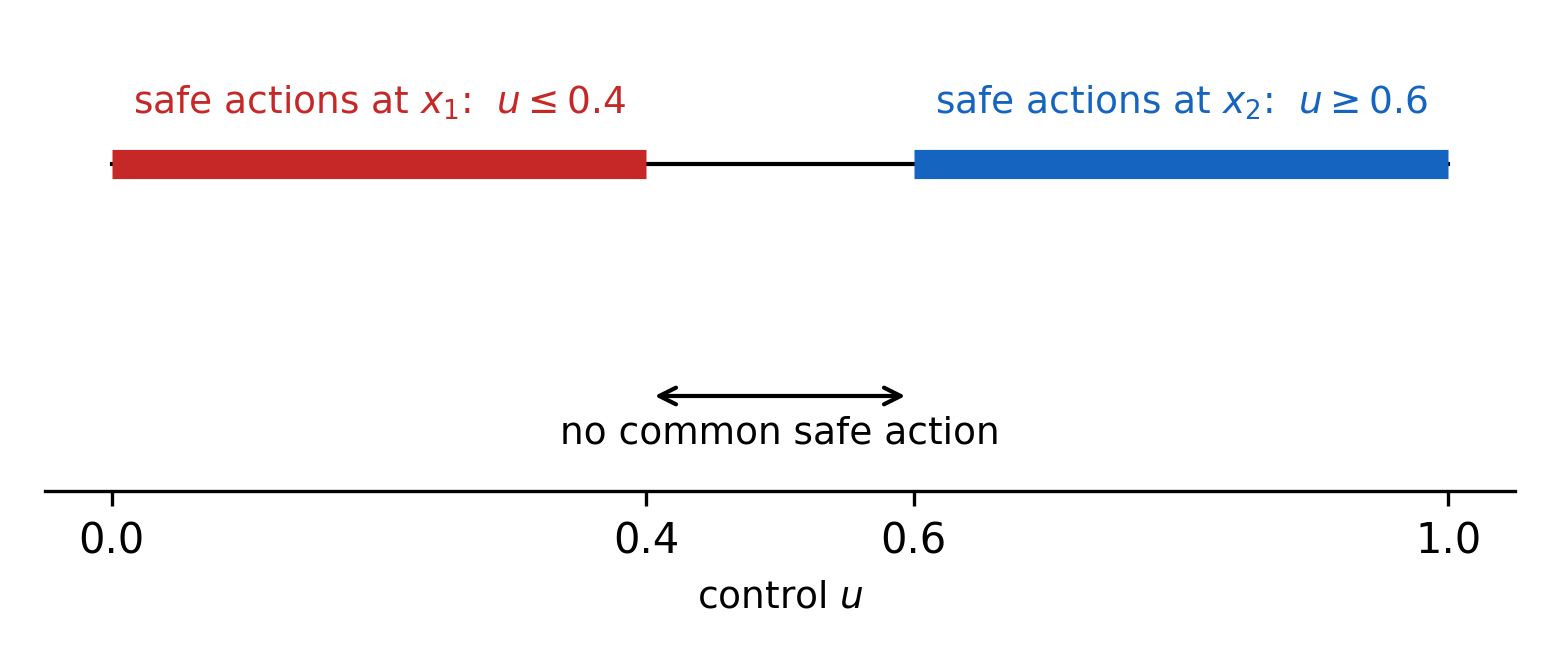
\includegraphics[width=0.82\columnwidth]{figs_p2/fig_p2_common_action.png}
\caption{Incompatible safe controls. The states \(x_1\) and \(x_2\)
share an observation, but their safe-action sets \([0,0.4]\) and
\([0.6,1]\) are disjoint, so no common safe action exists
(Theorem~\ref{thm:common-action}).}
\label{fig:common-action}
\end{figure}

\textbf{The tube-safety form.} The instantaneous condition (2) is the
\(\Delta \downarrow 0\) boundary approximation of the exact one-step
obstruction: with the action held over a review interval of length
\(\Delta\), the exact condition is the emptiness of the tube-safe action
set
\[\mathcal{A}_{\mathrm{tube}}(B, \Delta) \;=\; \Big\{ a : \mathrm{Reach}_{[0,\Delta]}(B, a) \subseteq \mathcal{V} \Big\},\]
with \(\mathrm{Reach}_{[0,\Delta]}(B, a)\) the robust (all-disturbance) reachable set (the reading specified in Section 2.4),
and \(\mathcal{A}_{\mathrm{tube}}(B, \Delta) = \varnothing\) certifies
\(B \notin \mathrm{ERViab}_{\mathcal{I}}(\mathcal{V})\) for every review
interval of length \(\Delta\) and every target collection. The theorems
above and below use the instantaneous and timing readings; the tube form
is the unifying one-step object.

\begin{proposition}[uniform margin gives a tube obstruction at every review length]\label{prop:uniform-margin}
Let \(B\subseteq\mathcal V\) be a compact information set with
\(U^B(B)\neq\varnothing\), \(f\) and \(\nabla q_j\) continuous, and
suppose there is \(\eta>0\) such that for every \(a\in U^B(B)\) there
exist a boundary state \(x_a\in B\cap\partial\mathcal V\), an active
constraint \(j\) with \(q_j(x_a)=0\), and a disturbance \(d_a\in D(x_a)\)
satisfying
\[\nabla q_j(x_a)\cdot f(x_a,a,d_a) \le -\eta.\]
Under the closed-loop existence convention of
Theorem~\ref{thm:common-action}, the tube-safe action set is then empty
at every review length,
\[\mathcal{A}_{\mathrm{tube}}(B,\Delta)=\varnothing \qquad \forall\,\Delta>0,\]
and hence \(B\notin\mathrm{ERViab}_{\mathcal I}(\mathcal V)\) under
sampled review of any length.
\end{proposition}

\emph{Proof sketch.} For fixed \(a \in U^B(B)\), continuity of the drift and the closed graph of \(D\) extend the margin to \(-\eta/2\) on a neighbourhood of \((x_a, a, d_a)\), and a measurable local selection realizes it; the trajectory from \(x_a\) under the held action then satisfies \(q_j(x(t)) \le -(\eta/2) t < 0\) for small \(t\), so \(a \notin \mathcal{A}_{\mathrm{tube}}(B, \Delta)\) for every \(\Delta > 0\). As \(a\) was arbitrary, the tube-safe action set is empty.

\begin{proposition}[obstruction ladder]\label{prop:ladder}
Under the standing regularity assumptions and the closed-loop existence
convention of Theorem~\ref{thm:common-action}, the common response sets
of Section 2.4 are nested:
\[\mathcal{A}_{\mathrm{tube}}(B,\Delta) \;\subseteq\; \mathcal{R}_{\mathcal{V}}^B(B) \;\subseteq\; U^B(B) \qquad \forall\,\Delta>0,\]
and emptiness descends the ladder:
\[
\begin{aligned}
U^B(B)=\varnothing \;&\Longrightarrow\; \mathcal{R}_{\mathcal{V}}^B(B)=\varnothing \;\Longrightarrow\; \mathcal{A}_{\mathrm{tube}}(B,\Delta)=\varnothing \\
&\Longrightarrow\; B\notin\mathrm{ERViab}_{\mathcal{I}}(\mathcal{V}).
\end{aligned}
\]
\end{proposition}

\emph{Proof sketch.} The inclusion \(\mathcal{R}_{\mathcal{V}}(x) \subseteq U(x)\) gives the second nesting. For the first, an action outside \(\mathcal{R}_{\mathcal{V}}^B(B)\) violates \(\nabla q_j(x) \cdot f(x, a, d) \ge 0\) at some active boundary state, and the corresponding trajectory leaves \(\mathcal{V}\) in arbitrarily small time, so the action is not tube-safe.

\textbf{The obstruction ladder.} Each certificate is a sufficient
condition for emptiness at one rung:
\begin{itemize}
\item \emph{Admissibility obstruction} --- \(U^B(B)=\varnothing\): no
single action is admissible at every compatible state (the base case of
Proposition~\ref{prop:emptiness}).
\item \emph{Common safe-action obstruction} ---
\(\mathcal{R}_{\mathcal{V}}^B(B)=\varnothing\) with
\(U^B(B)\neq\varnothing\) (the safety case of
Theorem~\ref{thm:common-action}).
\item \emph{Tube obstruction} ---
\(\mathcal{A}_{\mathrm{tube}}(B,\Delta)=\varnothing\) (the tube-safety
form).
\item \emph{Recursive obstruction} --- in the finite-horizon setting the
\(N\)-step common safe-action sets \(\mathcal{A}_N(B)\) of Section 3.1 complete the ladder
\(\mathcal{A}_N(B)\subseteq\mathcal{A}_{\mathrm{tube}}(B,\Delta)\subseteq\mathcal{R}_{\mathcal{V}}^B(B)\subseteq U^B(B)\).
\end{itemize}
The rungs are strict in general: \(\mathcal{R}_{\mathcal{V}}^B(B)\neq\varnothing\)
does not imply \(\mathcal{A}_{\mathrm{tube}}(B,\Delta)\neq\varnothing\)
for \(\Delta>0\), since an instantaneously tangent action may still exit
in finite time --- the gap that Proposition~\ref{prop:uniform-margin}
closes under a uniform margin. The dynamic exit certificate of
Theorem~\ref{thm:exit} sits below the ladder: it empties the response
set at some compatible state even under full information, which is the
strongest form of obstruction and needs no observation-theoretic
argument; the ladder, and the position of the exit certificate below it, are drawn in the Supplementary Material (Figure~S1).



\begin{example}[hidden-mode conflict]\label{ex:hidden-mode} Let an unobserved parameter satisfy
\(\theta \in \{-1, +1\}\), with \(\dot z = \theta u\),
\(u \in \{-1, +1\}\), and constraint \(z \ge 0\). At \(z = 0\): if
\(\theta = +1\), only \(u = +1\) is safe; if \(\theta = -1\), only
\(u = -1\) is safe. Both compatible states are individually robustly
viable under full information (each admits its safe control), but the
information set \(B = \{(0, +1), (0, -1)\}\) satisfies
\(\mathcal{R}_{\mathcal{V}}^B(B) = \{+1\} \cap \{-1\} = \varnothing\),
so \(B \notin \mathrm{ERViab}_{\mathcal{I}}(\mathcal{V})\). This is a
purely informational failure: no stochasticity and no estimation-quality
argument is involved. The example is the two-action skeleton of every
``the stock is either recovering or collapsing, and the safe policy
differs between the two'' situation.

\end{example}

\subsubsection{3.3 The delayed-information
obstruction}\label{the-delayed-information-obstruction}

\begin{theorem}[delayed-information obstruction]\label{thm:delayed}

Let \(B_0\) be an initial information set. Suppose the following
hypotheses hold.

(H4.1) No informative observation arrives before time
\(T_{\mathrm{obs}} > 0\) --- formally, there are branches that are
\textbf{observation-equivalent on \([0, T_{\mathrm{obs}})\)}: they
produce identical observation records throughout that interval, so the
policy cannot distinguish them before \(T_{\mathrm{obs}}\); between
observations the information set evolves by the set-membership semantics
of Section 2.3.

(H4.2) There exist a constraint function \(q\) of class \(C^1\) (the
class of Theorem~\ref{thm:exit}'s proof) with \(\mathcal{V} \subseteq \{ q \ge 0 \}\)
and a constant \(\varepsilon > 0\) such that, \textbf{for every implementable blind-window control} --- every
measurable \(u(\cdot)\) on \([0, T_{\mathrm{obs}})\) that is admissible at
every compatible state throughout the blind window, \(u(t) \in U^B(B_t)\)
with \(B_t\) the set-membership belief propagated under \(u(\cdot)\) ---
which is exactly the class of controls that an observation-based policy
can realize before the first informative observation, where its actions
are a fixed function of time --- there are a compatible initial state \(x^* \in B_0\) attaining
\(q(x^*) = \inf_{x \in B_0} q(x)\) (with \(B_0\) compact and \(q\) lower
semicontinuous; otherwise replace the infimum by \(\inf q + \delta\) for
an arbitrary \(\delta\)-minimizer, let \(\delta \downarrow 0\), and read
the timing bound with \(\inf q + \delta\)) and an admissible disturbance
realization such that, along the realized trajectory from \(x^*\) under
that open-loop control, the record remains compatible and
\[D^+ q(x(t); f(x(t), u(t), d(t))) \;\le\; -\varepsilon \qquad \text{while } q(x(t)) > 0, \tag{3}\]

(H4.3) The timing bound holds:
\[T_{\mathrm{obs}} \;>\; \frac{\inf_{x \in B_0} q(x)}{\varepsilon}. \tag{4}\]

Then, under hypotheses (H4.1)--(H4.3),
\(B_0 \notin \mathrm{ERViab}_{\mathcal{I}}(\mathcal{V})\): information
may be accurate but arrive too late.

\end{theorem}

\emph{Proof sketch.} By (H4.1) the policy's actions on \([0, T_{\mathrm{obs}})\) form one fixed open-loop control; if it is ever inadmissible at a compatible state the policy fails outright, otherwise (H4.2), applied to this implementable control, supplies a compatible state \(x^*\) with \(q(x^*) = \inf_{B_0} q\) and an admissible disturbance realizing the drift (3); integrating (3) gives \(q(x(t)) \le \inf_{B_0} q - \varepsilon t\), so the violation \(q < 0\) occurs by time \(\inf_{B_0} q / \varepsilon\), which (4) places strictly before \(T_{\mathrm{obs}}\) --- before any informative observation, so the policy cannot react in time.

The hypothesis (3) is the set-membership form of the drift condition,
quantified over open-loop controls on the blind window --- a condition
on the data of the problem, not on the policies: for every such control
there is a compatible state and disturbance enforcing the drift; the
adversary selects the true state and the disturbance, and the
observations cannot expose the selection in time. It is this open-loop form that gives the timing bound (4) its force --- (H4.1) converts
the policy's actions into one open-loop control, (H4.2) supplies the
drift against it, and (4) then makes the obstruction epistemic rather
than dynamic. The hypothesis is checkable in its special cases (constant
observations; hold-until-\(T_{\mathrm{obs}}\) policies) and is a template to be instantiated in the general case. Condition (4) is
the \textbf{timing bound}: it states that the observation arrives
\emph{after} the enforced exit time --- the cause of the obstruction; inverted, it reads as the design requirement that the first informative observation precede the enforced exit time
\(\inf q / \varepsilon\). Theorem~\ref{thm:delayed} complements Theorem~\ref{thm:common-action} quantitatively:
the common-action obstruction is a \textbf{formal zero-margin counterpart}
of the delayed tube-safety obstruction, and the two certificates remain
distinct --- the one a local action-feasibility condition, the other a
finite-time survival-value condition --- so the pair is not related as a
\(T_{\mathrm{obs}} \to \infty\) limit. It is the obstruction that
governs discrete-review governance: a review interval longer than the
worst-case exit time is an information structure in which the exit is inevitable.

\begin{remark}[threshold form of the timing obstruction]\label{rem:sigma}
The delayed-information obstruction has a sharp threshold. Let
\(\sigma^*(B_0)\) be the guaranteed blind-window survival time: the
largest duration such that some pre-observation policy keeps every
observation-equivalent branch in \(\mathcal{V}\) until then,
\[\sigma^*(B_0) \;=\; \sup_{u(\cdot)} \inf_{x_0\in B_0,\, d(\cdot)} \tau(x_0,u,d),\]
with the infimum over branches that remain observation-equivalent on
\([0,T_{\mathrm{obs}})\) and \(\tau\) the first violation time under the
convention of Theorem~\ref{thm:delayed}. Then
\[\sigma^*(B_0) < T_{\mathrm{obs}} \;\Longrightarrow\; B_0 \notin \mathrm{ERViab}_{\mathcal{I}}(\mathcal{V}),\]
because before \(T_{\mathrm{obs}}\) a policy cannot condition its action
on which branch realizes. Condition (4) certifies this threshold: under
(H4.1)--(H4.2) every branch exits by time
\(\inf_{x\in B_0}q(x)/\varepsilon\), hence
\(\sigma^*(B_0)\le\inf_{x\in B_0}q(x)/\varepsilon\), and (4) states that
this upper bound lies below \(T_{\mathrm{obs}}\); the threshold itself
may be strictly smaller, in which case nonviability holds even when (4)
fails. The threshold is the blind-window response correspondence of the
timing layer: its emptiness is the timing certificate, the
delayed-information analogue of the tube and common-action
correspondences.
\end{remark}

\begin{figure}[htbp]
\centering
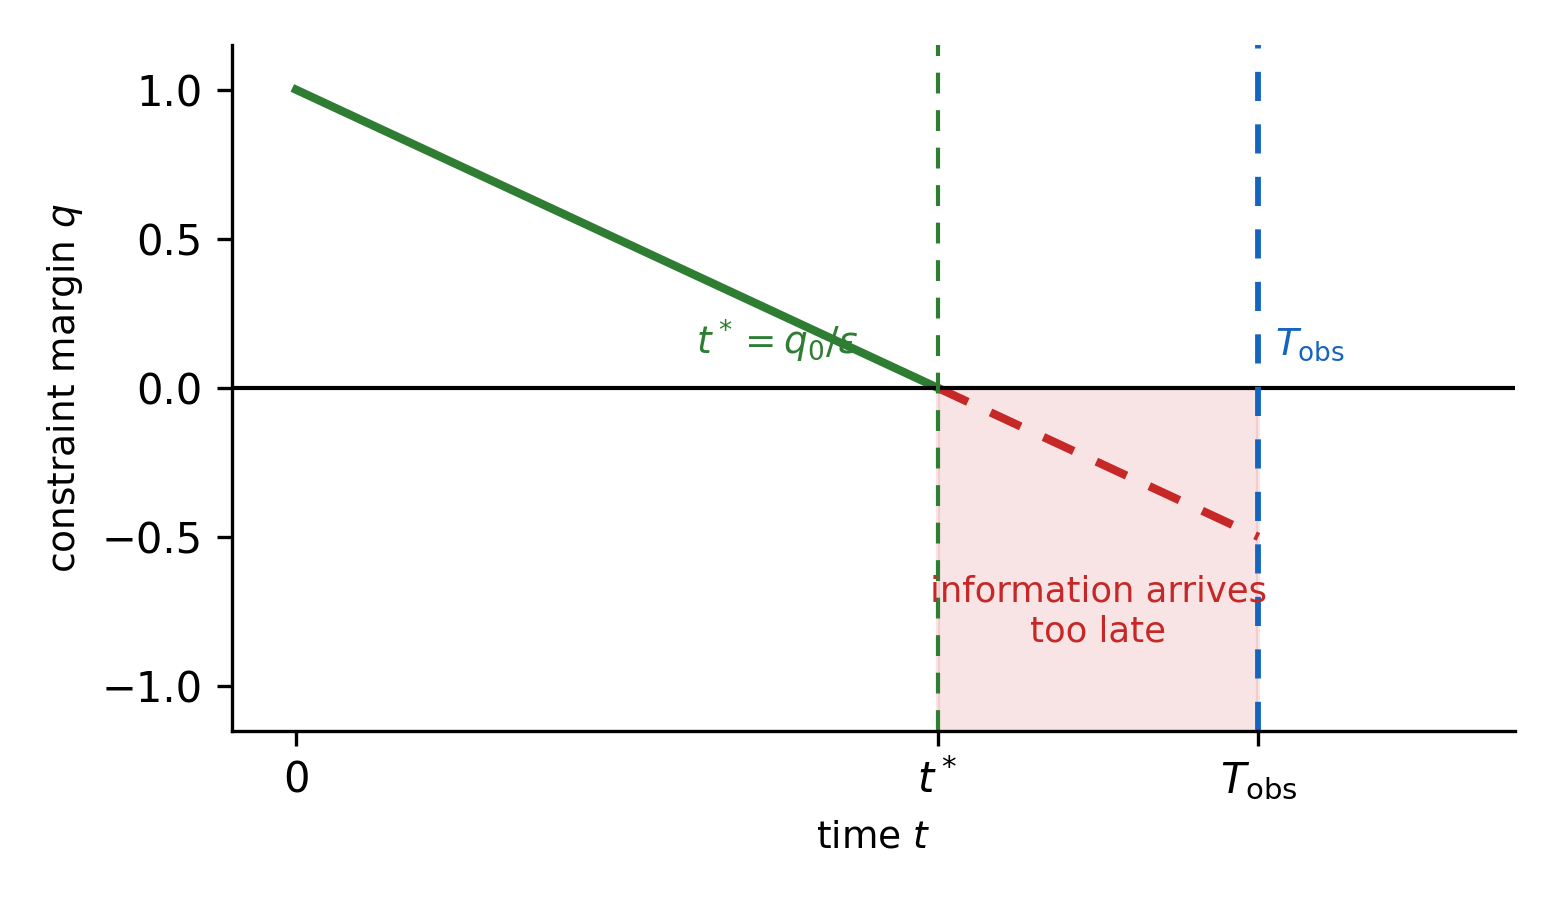
\includegraphics[width=0.82\columnwidth]{figs_p2/fig_p2_timing.png}
\caption{Delayed information. The constraint margin \(q\) reaches zero at
\(t^*=q_0/\varepsilon\), before the first informative observation at
\(T_{\mathrm{obs}}\): the information is accurate but arrives too late
(Theorem~\ref{thm:delayed}).}
\label{fig:timing}
\end{figure}

\subsubsection{3.4 The sparse finite
witness}\label{the-sparse-finite-witness}

\begin{proposition}[sparse common-action witness]\label{prop:helly}
Let \(B\subseteq\mathcal V\) be an information set, \(U(x)\subseteq U\)
with \(U\subseteq\mathbb R^m\) compact and convex and \(U(x)\) convex and
closed, let the dynamics be affine in the control,
\(f(x,u,d)=f_0(x,d)+f_u(x,d)\,u\), with \(D(x)\) compact, and let
\(\mathcal V\) have \(C^1\) constraint functions \(q_j\). Then each
safe-control set \(\mathcal R_{\mathcal V}(x)\) is a compact convex
subset of \(U\), and the safety-case common-action obstruction
\(\bigcap_{x\in B}\mathcal R_{\mathcal V}(x)=\varnothing\) holds if and
only if it is witnessed by at most \(m+1\) compatible states: there
exist \(x_1,\dots,x_{m+1}\in B\) with
\(\bigcap_{i=1}^{m+1}\mathcal R_{\mathcal V}(x_i)=\varnothing\). The
admissibility analogue (with \(\mathcal R_{\mathcal V}(x)\) replaced by
\(U(x)\)) holds under the same convexity assumptions.
\end{proposition}

\textbf{Proof.} For fixed \((x,j,d)\) the inequality
\(\nabla q_j(x)\cdot f(x,u,d)\ge 0\) is affine in \(u\), so
\(\mathcal R_{\mathcal V}(x)\), an intersection of closed halfspaces
(over active \(j\) and \(d\in D(x)\)) with the closed convex \(U(x)\),
is closed and convex; contained in the compact \(U\), it is compact. If
the intersection over all \(x\in B\) is empty, then by compactness some
finite subfamily of \(\{\mathcal R_{\mathcal V}(x)\}_{x\in B}\) already
has empty intersection, and by the finite Helly theorem at most \(m+1\)
members suffice; the converse direction is immediate. \hfill\(\square\)

\textbf{A worked certificate (two floors, one scalar action).} Two
floors demand incompatible extraction rates on a single control
\(u\in[0,1]\). At the compatible state \(x_1\) (floor 1 active) the safe
controls are \(u\le 0.4\); at \(x_2\) (floor 2 active) they are
\(u\ge 0.6\). The observation merges \(x_1\) and \(x_2\), so a common
safe action must satisfy both. Writing the constraints as \(Au\le b\)
with \(A=(1,-1)^{\top}\) and \(b=(0.4,-0.6)^{\top}\), the stacked system
\(u\le 0.4\), \(-u\le -0.6\) is infeasible; the Farkas certificate is
\(\lambda=(1/2,1/2)\) (normalized, \(\|\lambda\|_1=1\)), for which
\(\lambda^{\top}A=0\) and \(\lambda^{\top}b=-0.1<0\). Under the normalization
\(\|\lambda\|_1=1\), the magnitude \(|\lambda^{\top}b|=0.1\) is the
infeasibility margin of the stacked system, shrinking to zero exactly as
the two safe-action sets come to touch. The multiplier
exhibits the contradiction as a convex combination of the two floor
constraints: no common extraction rate respects both floors, and any
observation that separates \(x_1\) from \(x_2\) restores one-step
viability (Figure~\ref{fig:common-action}). With \(m=1\), the two
incompatible states are exactly the \(m+1\)-state witness of
Proposition~\ref{prop:helly}.

\subsubsection{3.5 The finite-time exit
certificate}\label{the-finite-time-exit-certificate}

The base obstruction operates before any observation-theoretic argument: it
certifies membership in the full-information ``shadow'' --- the
complement of the viability kernel (Aubin, 2001; Aubin and
Catt\'e, 2002).
It is a drift condition under which \emph{no} control --- of any
information structure --- can be viable. Put in management terms, when the dynamics themselves force exit before any control can react, no monitoring design can rescue viability, and the certification problem is closed without observation-theoretic reasoning.

\begin{theorem}[finite-time exit certificate]\label{thm:exit}

Let \(q : X \to \mathbb{R}\) be a constraint function of class \(C^1\) --- the class assumed throughout the exit theorems --- with
\(\mathcal{V} \subseteq \{ q \ge 0 \}\), and suppose the following
hypotheses hold.

(H1.1) There exist constants \(a > 0\) and \(\varepsilon > 0\) such that
on the strip \(\mathcal{S}_a = \{ x : 0 \le q(x) \le a \}\),
\[\sup_{u \in U(x)} \inf_{d \in D(x)} D^+ q(x; f(x,u,d)) \;\le\; -\varepsilon \qquad \forall x \in \mathcal{S}_a, \tag{1}\]
where \(D^+ q(x; v) = \limsup_{h \downarrow 0} [q(x + hv) - q(x)]/h\) is
the upper right Dini derivative of \(q\) in direction \(v\) (for \(C^1\)
\(q\), \(D^+ q(x; v) = \nabla q(x) \cdot v\) --- the form the proof
uses).

(H1.2) \textbf{Closed-loop existence of the adverse realization.} The
disturbance correspondence is lower semicontinuous, or constant, on the
strip, so that the state-dependent adverse selection constructed in the
proof is realized by an admissible control--disturbance pair for which
the Carath\'eodory existence theorem applies. (Alternatively, without (H1.2), the certificate is read against the convexified (relaxed) inclusion
\(\dot x \in \mathrm{co}\, f(x, u(t), D_{\varepsilon}(x, u(t)))\), which
admits solutions under Marchaud-type conditions and preserves the drift
inequality because, for \(C^1\) \(q\), the directional derivative
\(\nabla q(x)\cdot v\) is affine in the velocity; closure and
relaxation are the standard tools for this step.)

Then, under hypotheses (H1.1)--(H1.2), for every
admissible control and every initial state \(x_0 \in \mathcal{S}_a\)
there exists an admissible disturbance realization under which the
trajectory attains \(q(x(t)) < 0\) --- hence leaves
\(\{ q \ge 0 \} \supseteq \mathcal{V}\) --- by every time strictly
larger than \(q(x_0)/\varepsilon\):
\(\inf\{ t : q(x(t)) < 0 \} \le q(x_0)/\varepsilon\), in particular
within time at most \(a/\varepsilon\) (since \(q(x_0) \le a\)).
(Convention, used in both exit theorems: \emph{violation} is the strict
inequality \(q < 0\); at \(q = 0\) the state may still lie on
\(\partial \mathcal{V} \subseteq \mathcal{V}\).)

\end{theorem}

\emph{Proof sketch.} Fix an admissible control. By (1), the adverse-selection correspondence \(D_\varepsilon(x,u)\) has nonempty values on the strip; its closed graph and compact values (Section 2.1) yield a measurable selection \(d(\cdot)\), realized in closed loop by (H1.2). The fundamental theorem of calculus integrates (1) along the resulting trajectory to \(q(x(t)) \le q(x_0) - \varepsilon t\), so \(q\) attains the strict violation \(q < 0\) by time \(q(x_0)/\varepsilon \le a/\varepsilon\).

\begin{remark}[comparison-function form]\label{rem:comparison}
Hypothesis (H1.1) uses a constant drift margin \(\varepsilon\). The
certificate extends to state-dependent decline: if there is a continuous
\(\alpha:(0,a]\to(0,\infty)\) with
\[\sup_{u\in U(x)}\inf_{d\in D(x)} D^+q(x; f(x,u,d)) \le -\alpha(q(x)) \qquad \forall x\in\mathcal{S}_a,\]
then the exit-time bound sharpens to
\[t_{\mathrm{exit}} \le \int_0^{q(x_0)} \frac{ds}{\alpha(s)},\]
whenever the integral is finite. The proof replaces the linear comparison
\(q(x(t))\le q(x_0)-\varepsilon t\) with the solution \(r\) of
\(\dot r=-\alpha(r)\), \(r(0)=q(x_0)\), by the standard comparison
argument. If \(\alpha(0)=0\) and the integral diverges, the conclusion
weakens to asymptotic approach rather than finite-time exit; the
constant-margin case \(\alpha\equiv\varepsilon\) is the sharp finite-time
instance.
\end{remark}

Two readings of (1) matter. First, it is an \textbf{Isaacs-type
condition}: the disturbance chooses after the control, so the
certificate asserts that the disturbance can \emph{enforce} exit against
any policy. Second, (1) is an outward-drift certificate \emph{dual in
spirit, but not logically complementary}, to an inward barrier
condition. The pointwise robust barrier reading is
\(\sup_u \inf_d D^+ q \ge 0\) --- some control keeps the drift inward
against every disturbance --- and the two conditions leave an unresolved
intermediate region in which neither holds (Section 6.2). Theorem~\ref{thm:exit} is
the ``unsafety'' side of that duality, and it is unconditional: it needs
no observation argument because it defeats all controls, including
clairvoyant ones.

\subsubsection{3.6 Epistemic emptiness by admissibility: a minimal
construction}\label{epistemic-emptiness-by-admissibility-a-minimal-construction}

The remaining obstructions apply to systems in which every state is
individually viable under full information and the kernel empties only under the observation structure.
The minimal construction of this section empties the kernel through
\emph{admissibility} --- a state-dependent control set whose common
action is forced and unsafe at the boundary; the common-action
obstruction of Section 3.2 and Example~\ref{ex:hidden-mode}'s hidden-parameter
conflict are the informational cases proper, merging states with
incompatible safe controls. In ecological terms, each stock is manageable on its own; the failure arises because the indicator cannot tell the manager which stock is present.

\begin{proposition}[epistemic emptiness by admissibility --- a minimal construction]\label{prop:emptiness}

There exists a system with
\(\mathrm{Viab}(\mathcal{V}; U, \pi_{\mathrm{perf}}) = \mathcal{V} \neq \varnothing\)
such that, for a non-injective observation map \(O\), every admissible
initial information state --- the observation fibres
\(B_0 = O^{-1}(O(S_0))\), \(S_0 \in \mathcal{V}\) --- lies outside
\(\mathrm{ERViab}_{\mathcal{I}}(\mathcal{V})\): the epistemic kernel
over the fibre-induced initial beliefs is empty. The mechanism is \emph{admissibility} rather than a hidden mode: the
state-dependent control set of the construction leaves a single common
action at the merged belief --- one that is outward-drifting at the
boundary state --- so the emptiness is the common-action obstruction
(Theorem~\ref{thm:common-action}'s safety case) at minimal size, produced by the control-set primitive rather than by information; the
hidden-mode instance is Example~\ref{ex:hidden-mode}.

\end{proposition}

\emph{Proof sketch (construction).} Take \(X = [1,2]\), \(\dot S = u - r(S)\) with \(r\) continuous and injective, \(U(S) = \{0, r(S)\}\), \(\mathcal{V} = [1,2]\), and the constant observation \(O \equiv 0\). Under full information \(u = r(S)\) gives \(\dot S = 0\), so every state is viable. Under \(O \equiv 0\) the common control set over the fibre is \(\{0\}\) --- injectivity of \(r\) rules out a common \(r(S)\) --- so the policy must hold \(u = 0\), and \(\dot S = -r(S) < 0\) drives every compatible trajectory out of \(\mathcal{V}\) in finite time.

The construction isolates an admissibility mechanism: the observation merges states whose \emph{admissible}
controls differ --- the merged belief admits a common admissible control
(the singleton \(\{0\}\)) but no common \emph{safe} control, because
that singleton is outward-drifting at the boundary state \(S = 1\). The
``inadmissible action = failure'' convention is used explicitly: an action outside \(U(x)\) at a compatible state \(x\) is
itself failure, and the state-dependent control set
\(U(S) = \{0, r(S)\}\) is a modelling primitive carrying that convention
(Theorem~\ref{thm:common-action}'s admissibility case uses the same convention, stated there).
The example also shows the empty-kernel phenomenon at its minimal size
--- two control values, one scalar state --- as the minimal instance of
Theorem~\ref{thm:common-action} rather than a mechanism of equal rank; with a constant control
set \([0, \bar u]\) in the same plant the fibre is epistemically viable
(a constant control \(u = r(m)\), \(m \in (1,2)\), drives every state of
the fibre to the rest point \(m \in (1,2)\)), so the construction is an admissibility mechanism rather than a hidden-mode mechanism. Theorem~\ref{thm:common-action} states the general obstruction, of which this construction is
the minimal instance.

\subsection{4. Certification Limits}\label{certification-limits}

\subsubsection{4.1 Exact certification and the fibre
criterion}\label{exact-certification-and-the-fibre-criterion}

The obstruction theorems of Section 3 concern \emph{policies}.
Sustainability governance also uses \emph{certificates}: verdicts
--- safe or unsafe --- computed from observations alone, without
reference to a policy. The question is when such verdicts can be exact.
For a manager operating under partial ecological information, the question is whether an indicator reading alone can ever settle whether the system is on the safe side of a specified floor.

\begin{definition}[exact certifier]\label{def:certifier}

For an admissible domain
\(Z \subseteq X\) and a safe set \(K \subseteq Z\), an \textbf{exact
certifier} based on the observation map \(O : Z \to Y\) is a function
\(C : Y \to \{0,1\}\) such that
\[C(O(z)) = 1 \iff z \in K \qquad \text{for every } z \in Z.\]

\end{definition}

\begin{proposition}[observation-fibre criterion]\label{prop:fibre}

An exact certifier
based on \(O\) exists if and only if membership in \(K\) is constant on
every observation fibre:
\[O(z_1) = O(z_2) \;\Longrightarrow\; \big[ z_1 \in K \iff z_2 \in K \big] \qquad \forall z_1, z_2 \in Z, \tag{5}\]
equivalently, \(K = O^{-1}(O(K))\) on the admissible domain.

\end{proposition}

\emph{Proof sketch.} If \(C\) exists and \(O(z_1) = O(z_2)\), then \(\mathbf{1}_K(z_1) = C(O(z_1)) = C(O(z_2)) = \mathbf{1}_K(z_2)\), so membership is fibre-constant. Conversely, (5) makes \(C(y) = \mathbf{1}_K(z)\) for any \(z\) with \(O(z) = y\) well defined and exact.

The fibre criterion concerns static classification --- whether
membership in a safe set factors through the observation --- and applies
verbatim to three distinct certification problems, which should not be
conflated: constraint certification (\(K = \mathcal{V}\)), robust
viability certification (\(K = \mathrm{RViab}(\mathcal{V})\)), and
policy-specific safety certification (\(K = \mathrm{Safe}^{\Pi}_T\)).
The same theorem governs all three, but its governance meaning differs.
The criterion is the zero-step, label-valued analogue of the
common-action test: an observation-based verdict assigns a single label
to an entire fibre, exactly as an observation-based action assigns a
single action to an entire belief, so both are selector problems. They
remain distinct --- a fibre may fail exact certification while a policy
is still viable, and exact static certification does not imply dynamic
viability; hence certification is treated as a layer separate from
viability throughout.

\begin{corollary}[safety-crossing fibres and the certainly-safe set]\label{cor:certainly-safe} If two admissible states share an observation and lie on opposite
sides of the \emph{same} component safety constraint --- with the safe
set of that certification problem read as the single floor
\(K = \{ q_j \ge 0 \}\); or, in the general form of the hypothesis, one
of the two states lies in \(K\) and the other outside \(K\) --- no exact
observation-only certificate exists. (Crossing one floor of an
intersection \(K = \bigcap_j \{ q_j \ge 0 \}\) does not by itself put
the pair on opposite sides of the intersection --- the state satisfying
floor \(j\) may violate floor \(i\) --- hence the single-floor scoping.)
The largest set of observations that can soundly be labeled safe without
further information is the certainly-safe set
\[\mathcal{Y}_{\mathrm{safe}} \;=\; \big\{ y \in O(Z) : O^{-1}(y) \subseteq K \big\}.\]

\end{corollary}

\emph{Proof sketch.} A fibre containing one state in \(K\) and one outside violates (5), so Proposition~\ref{prop:fibre} denies the certifier. On \(\mathcal{Y}_{\mathrm{safe}}\) every compatible state is safe, so the constant verdict ``safe'' is sound; outside it some compatible state is unsafe, so no sound ``safe'' verdict exists.

The fibre criterion has a direct governance reading. A composite
sustainability index is an observation map from the state of a
socio-ecological system to a scalar; a floor is a safe set. Corollary~\ref{cor:certainly-safe}
then states: an index whose fibres cross a floor boundary --- whose
value cannot distinguish a state violating the floor from one satisfying
it --- cannot support an exact certification of that floor, however
carefully the index is thresholded. The structural requirement is not
that each floor be measured separately, but that the observation
\emph{separate every admissible pair lying on opposite sides of a specified floor}; direct per-floor measurement is one sufficient design,
not the unique one, and any statistic refining the floor's safe/unsafe
partition certifies equally well. The certainly-safe set is the sound relaxation: it is the set of observation values where the index may certify safety; outside
it, the index must fall silent.

\begin{figure}[htbp]
\centering
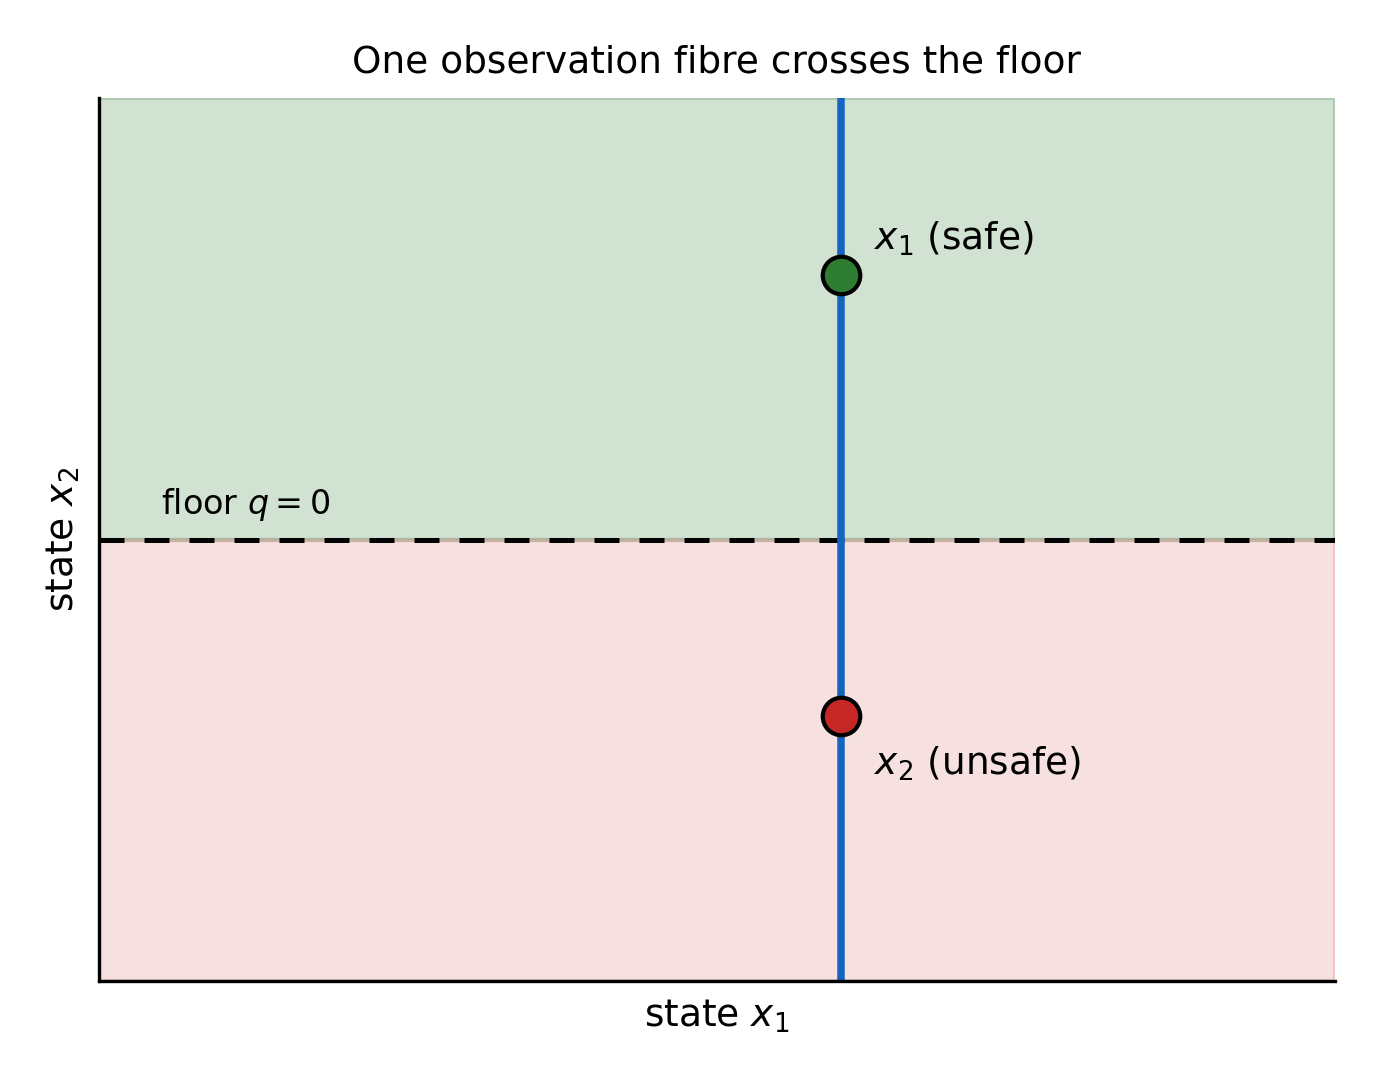
\includegraphics[width=0.82\columnwidth]{figs_p2/fig_p2_fibre.png}
\caption{An observation fibre crossing a floor boundary. The observation
\(O(x)=x_1\) cannot separate the safe state \((0.6,0.8)\) from the unsafe
state \((0.6,0.3)\) on the same fibre, so no exact observation-only
certifier exists (Proposition~\ref{prop:fibre}).}
\label{fig:fibre}
\end{figure}

\subsubsection{4.2 The certainty-equivalence
trap}\label{the-certainty-equivalence-trap}

The obstruction of Proposition~\ref{prop:emptiness} relies on a non-injective observation ---
information lost. The same emptying occurs with a fully
\emph{injective} observation for a single policy: the canonical
certainty-equivalence controller that applies a perfect-information law
to the uncorrected observation.

\begin{remark}[the certainty-equivalence trap]\label{rem:ce-trap}

Consider \(\dot S = u - g(S)\) with \(u \in [0, \bar u]\), \(g\) strictly
increasing on \([S_{\min}, S^* + b]\), \(g(0) = 0\), and
\(\mathcal{V} = [S_{\min}, S^*]\). Assume the range condition
\(g(S + b) \le \bar u\) for every \(S \in [S_{\min}, S^*]\), so that the
controller below is admissible. Under perfect information the zeroing
feedback \(u(t) = g(S(t))\) gives \(\dot S = 0\), so every
\(S_0 \in \mathcal{V}\) is viable and
\(\mathrm{Viab}(\mathcal{V}; U, \pi_{\mathrm{perf}}) = \mathcal{V} \neq \varnothing\).
Now take the injective, biased observation \(\hat S = S + b\) with
\(b > 0\), and the canonical certainty-equivalence controller: the
perfect-information zeroing law applied directly to the uncorrected
observation, \(u = g(\hat S) = g(S + b)\). Then
\[\dot S = g(S + b) - g(S) > 0 \qquad \forall S,\]
and since \(g\) is strictly increasing on the compact interval
\([S_{\min}, S^* + b]\), \(\dot S\) is bounded below by a positive
constant there; hence \(S\) strictly increases and exits above \(S^*\) in
finite time from every \(S_0 \in \mathcal{V}\): the kernel of this single
controller is empty. The bias-corrected controller
\(u = g(\hat S - b) = g(S)\) uses the observation map's structure, restores
\(\dot S = 0\), and keeps the kernel nonempty.

The mechanism is a \emph{failure of one policy to use the observation
map's structure}, not a loss of information: for a known invertible
observation the output-feedback class is as powerful as the
state-feedback class. The phenomenon is the viability-theoretic analogue
of Witsenhausen's counterexample in stochastic control (Witsenhausen,
1968): the information pattern --- not the dynamics and not the
constraint --- defeats the uncorrected controller. The remark is
policy-specific; it does not assert that the entire certainty-equivalence
class empties the kernel.

\end{remark}





\subsection{5. The Sufficiency Landscape}\label{the-sufficiency-landscape-cited}

For contrast, we record the sufficiency results against which the obstruction calculus is defined; the proofs are in the cited sources.

\textbf{(a) Veliov's output-feedback condition.} Veliov (1993) gives a sufficient condition for the existence of an output-feedback regulation map under incomplete and inexact measurement, reducing under perfect measurement to the classical viability condition (Haddad, 1981). Veliov's theorem certifies existence; the obstruction calculus certifies nonexistence; a problem satisfying neither requires a stronger observer or a finer observation structure.

\textbf{(b) The estimation-tube programme.} Cardaliaguet, Quincampoix, and Saint-Pierre (2007) pass from imperfect information in the measurement space to perfect information in an estimation space of sets of compatible states, with equality of value functions and a Dini-derivative characterization. Under the set-membership semantics the estimation-space solution propagates the belief under a single control signal, so its controls are common controls; the common-action obstruction (Theorem~\ref{thm:common-action}) is the certificate that no jointly admissible selection exists at the information state in question (Section 6.3).

\textbf{(c) Observer-and-buffer transfer.} If a full-information feedback exists with a strict inward margin and an observer supplies exponentially convergent estimates, output feedback of the estimate preserves safety on a buffered subset (observer-to-viability transfer with safety buffer; Sontag, 1998), and eroded kernels remain invariant under bounded estimation and implementation errors (erosion absorbs the error). Under margins and convergence, output feedback can work; Sections 3--4 state when it cannot.

\textbf{(d) The linear substitution alternative.} For a finite linear model in which a resource-typed system must meet a demand vector through specified substitution pathways, exactly one of the following holds (Farkas, 1902; Gale, 1960): (i) there exists a non-negative pathway vector \(a \ge 0\) satisfying the linear substitution constraints; or (ii) there exist multipliers \(\alpha, \beta, \gamma \ge 0\) with
\[
\begin{aligned}
&\alpha^\top R + \beta^\top E - \gamma^\top Q \ge 0 \quad\text{componentwise},\\
&\gamma^\top s^{\mathrm{req}} > \alpha^\top x + \beta^\top e.
\end{aligned}
\]
The second statement is a separation certificate that the pathways cannot meet demand within the typed resource and capacity bounds --- the feasibility-side complement of the observation-side obstructions of Sections 3--4.
\subsection{6. Discussion}\label{discussion}


\subsubsection{6.1 The shape of the
calculus}\label{the-shape-of-the-calculus}

The six mechanisms form a nonexhaustive taxonomy of information-theoretic failure. Table~\ref{tab:summary} collects the certificates, the response correspondence each one empties, and the design consequence each one licenses.

\begin{table*}[t]
\centering
\footnotesize
\begin{tabular}{@{}l>{\raggedright\arraybackslash}p{3.4cm}>{\raggedright\arraybackslash}p{4.4cm}@{}}
\toprule
Certificate & Emptied response correspondence & Design consequence (Section 6.4) \\
\midrule
finite-time exit (Theorem~\ref{thm:exit}) & the response set of some compatible state, even under full information & none --- dynamics, not information \\
admissibility (Proposition~\ref{prop:emptiness}) & \(U^B(B)=\varnothing\) & enlarge the command set \\
common action and tube (Theorem~\ref{thm:common-action}, Proposition~\ref{prop:uniform-margin}) & \(\mathcal{R}_{\mathcal{V}}^B(B)=\varnothing\), \(\mathcal{A}_{\mathrm{tube}}(B,\Delta)=\varnothing\) & a separating observation; a shorter review interval \\
delayed information (Theorem~\ref{thm:delayed}, Remark~\ref{rem:sigma}) & \(\sigma^*(B_0)<T_{\mathrm{obs}}\) & an earlier informative observation \\
fibre certification (Proposition~\ref{prop:fibre}, Corollary~\ref{cor:certainly-safe}) & \(K\neq O^{-1}(O(K))\) & a refined index; per-floor measurement \\
certainty equivalence (Remark~\ref{rem:ce-trap}) & kernel of the uncorrected controller \(u=g(\hat S)\) is empty & correct the known bias \\
finite-horizon recursion (Theorem~\ref{thm:finite-horizon}) & \(B_0\notin\mathcal{W}_N\) & exact characterization (Section 3.1) \\
\bottomrule
\end{tabular}
\caption{The obstruction certificates, the response correspondence each one empties, and the design consequence each one licenses. The first six are sound sufficient conditions for nonviability; the last is the exact finite-horizon characterization.}
\label{tab:summary}
\end{table*} The exit certificate (Theorem~\ref{thm:exit}) is the
dynamic obstruction: it defeats all controls, so it needs no observation
argument. The epistemic-emptiness construction (Proposition~\ref{prop:emptiness}) exhibits the
mechanism at minimal size --- one scalar state, two admissible controls,
one constant observation --- in the admissibility form of Section 3.6. The common-action obstruction (Theorem~\ref{thm:common-action}) is the static
obstruction: it defeats all policies at a single information state. The
delayed-information obstruction (Theorem~\ref{thm:delayed}) interpolates between them in
time. The fibre criterion (Proposition~\ref{prop:fibre}) is the certification obstruction:
it limits not policies but verdicts. The certainty-equivalence trap
(Remark~\ref{rem:ce-trap}) limits a single uncorrected policy. Finite-horizon completeness
(Theorem~\ref{thm:finite-horizon}) supplies the exact finite-setting
counterpart of these sufficient certificates.

A governance failure of observation can be diagnosed by which
certificate applies. If the exit certificate holds, no monitoring design
helps --- the dynamics are adverse under every control. If only the
common-action obstruction holds, the remedy is a finer observation
structure (an informative measurement distinguishing the incompatible
states). If the delayed-information obstruction holds with a slack
timing bound, the remedy is a shorter review interval or a faster
indicator. If the fibre criterion fails, the remedy is an observation
that separates the sides of the floor rather than a better threshold on
the aggregate.

\subsubsection{6.2 Relation to barrier
certificates}\label{relation-to-barrier-certificates}

Barrier certificates certify safety from a scalar function whose zero level set separates the unsafe region from all trajectories (Prajna and Jadbabaie, 2004; Prajna, Jadbabaie, and Pappas, 2007); the converse, under convex-duality conditions on density functions, is Prajna and Rantzer (2005), and necessary-and-sufficient hybrid characterizations are Maghenem and Sanfelice (2019). Theorem~\ref{thm:exit} is the unsafety complement of that converse, not its observation-theoretic counterpart: a Dini-drift certificate of unsafety needing no observation structure, constructive in the enforcing disturbance and exit time. The remaining certificates (Proposition~\ref{prop:emptiness}, Theorem~\ref{thm:common-action}, Theorem~\ref{thm:delayed}, Proposition~\ref{prop:fibre}) act at the level of the information set itself: barrier constructions presuppose a state --- or a specified state estimate --- for feedback, whereas the common-action and timing obstructions certify the emptiness of the common safe-action set at a given information state, which barrier methods do not address.

The estimation-tube programme shows that imperfect measurement can be absorbed into set-valued dynamics on an estimation space with no loss in value (Cardaliaguet, Quincampoix, and Saint-Pierre, 2007); the present theorems delimit its reach rather than contradict it. The reduction preserves values, and its belief-state controls are common controls; the obstruction calculus is the local certificate layer of that programme --- the common-action obstruction certifies that the belief-state predecessor is empty, the timing bound quantifies when it fails for reasons of information arrival, and the fibre criterion states when no observation-based verdict can be exact. Belief-space viability answers \emph{whether}; the obstruction calculus answers \emph{why not, and what to change}.

\subsubsection{6.4 Consequences for monitoring and indicator
design}\label{consequences-for-monitoring-and-indicator-design}



Five consequences follow directly from the certificates. Each translates
a formal impossibility into a concrete design specification for
monitoring systems under partial ecological information.

\textbf{Timing.} Theorem~\ref{thm:delayed} gives the minimal monitoring frequency in
closed form: the first informative observation must precede the enforced
exit time \(\inf q / \varepsilon\). A review interval longer than the
worst-case time from the most-constrained compatible state --- the
minimum-\(q\) state, which has the least constraint slack --- to
constraint violation is an information structure under which the
violation is undetectable in time, whatever the review then concludes.
The bound is computable from the drift certificate (3), which a robustness analysis computes in any case.

\textbf{Coarseness.} Theorem~\ref{thm:common-action} states that an observation structure
merging two compatible states with incompatible safe controls is
nonviable \emph{at that information state}, even though both states are
viable in isolation. The design consequence is that the observation must
separate safety classes, not states: an indicator is exposed to Theorem~\ref{thm:common-action}'s obstruction when some observation fibre crosses the safe-control
partition of the state space --- merging states whose safe controls differ is what the theorem certifies, and keeping every fibre within a single class is what removes that exposure; refinement is never harmful (a finer observation merges nothing the coarser one did not), though Theorem~\ref{thm:common-action}
claims no benefit beyond the removal, and other mechanisms may still
certify nonviability on a finer partition.

\textbf{Aggregation.} Proposition~\ref{prop:fibre} and Corollary~\ref{cor:certainly-safe} apply verbatim to
composite indices, which are observation maps from the system state to a
scalar. An index whose fibres cross a floor boundary cannot support
exact floor certification; the certainly-safe set is the domain in which an index-based verdict is sound. Where separately-binding floors matter, exact
certification requires an observation that separates every admissible
pair on opposite sides of a floor (per-floor measurement is one sufficient design), a formal complement to the thesis, argued informally since Martinez-Alier, Munda, and O'Neill (1998), that weakly comparable
values cannot be fused into one metric without loss. The requirement is
sharpest where the floor constrains the productive base rather than its
output: an aggregate of services can read at full level while the base
regenerating them is reduced beneath it, and only an observation
reaching the base itself can detect the discrepancy.

\textbf{Bias.} Remark~\ref{rem:ce-trap} shows that the loss need not be in the
measurement: a biased indicator with an uncorrected
certainty-equivalence policy empties the epistemic kernel of a system
whose perfect-information kernel is nonempty. Monitoring therefore has
two obligations --- bounding the observation error and supplying the
correction --- and the second is the one governance structures can omit: the indicator is published, the correction is not applied,
and the kernel empties although the information was sufficient.

\textbf{Institutions.} The hierarchy of Section 2.1 records that
epistemic contraction is one of three causes of kernel shrinkage, the
others being disturbances and institutional restriction (authority,
enforcement, allocation). The epistemic-institutional kernel \(\mathrm{IRViab}_{\mathcal{J}}(\mathcal{V})\) (Section 2.1) combines them: an institution restricted in what it
may observe \emph{and} in what it may command inherits both
contractions. The obstruction calculus characterizes the first; its certificates remain valid, and typically tighten, when the institution's command set is further restricted, since restriction of
the action correspondence can only empty kernels, never create them
(one-sided monotonicity of viability under correspondence restriction).

\begin{proposition}[monotonicity of the epistemic kernel]\label{prop:monotone}
The robust epistemic kernel is monotone in its constituents: enlarging
the action sets, reducing the disturbance sets, refining the information
structure, or enlarging the policy class never shrinks the kernel.
Writing \(\mathrm{ERViab}^{\,\cdot}\) for the kernel with the indicated
constituent, \(U_1\subseteq U_2\), \(D_1\subseteq D_2\),
\(\Pi_1\subseteq\Pi_2\), and ``\(\mathcal{I}_1\) refines
\(\mathcal{I}_2\)'' imply respectively
\[\mathrm{ERViab}^{U_1} \subseteq \mathrm{ERViab}^{U_2}, \qquad
\mathrm{ERViab}^{D_2} \subseteq \mathrm{ERViab}^{D_1},\]
\[\mathrm{ERViab}^{\Pi_1} \subseteq \mathrm{ERViab}^{\Pi_2}, \qquad
\mathrm{ERViab}^{\mathcal{I}_2} \subseteq \mathrm{ERViab}^{\mathcal{I}_1}.\]
\end{proposition}

\emph{Proof sketch.} A policy viable under the smaller action sets, larger disturbance sets, smaller policy class, or coarser information structure remains admissible and nonanticipative under the corresponding enlargement or refinement, while the adversary's options are unchanged or reduced; the same policy witnesses viability.

\subsubsection{6.5 Limitations}\label{limitations}

The certificates are sound but not complete; several extensions are noted as open.

\begin{enumerate}
\def\labelenumi{(\roman{enumi})}
\tightlist
\item
  The continuous-time certificates of Sections 3.2--3.3 and 3.5--3.6 are sufficient conditions for nonviability, not necessary-and-sufficient characterizations of the epistemic kernel (backward recursion is complete in the finite-horizon finite-system setting, Section 3.1); the middle ground (neither a Veliov-type condition nor an obstruction certificate) is open. In
continuous settings completeness would additionally require a
measurable-selection theory beyond the explicit selections the
certificates exhibit; completeness is therefore claimed only where
backward recursion is exact (Section 3.1).
\item
  The timing obstruction of Theorem~\ref{thm:delayed} (and its threshold form, Remark~\ref{rem:sigma}) certifies failure by exit \emph{before} the first informative observation. It is blind to the complementary mode of nonviability --- \emph{insufficient post-observation recourse} --- in which a common blind-window control keeps every compatible branch safe, yet no observation-adapted control can recover every branch once the distinguishing observation arrives; the finite-horizon recursion (Section 3.1) captures that mode, but no continuous-time certificate for it is supplied here.
\item
  The information-set semantics is set-membership; probabilistic or belief-space formulations require separate statements, although the common-action obstruction transfers mutatis mutandis to any semantics in which the policy must choose a single action per information state.
\item
  The results are finite-dimensional and time-invariant; the delay-free setting makes the timing bound of Theorem~\ref{thm:delayed} sharp, and delay systems require the retarded extension of the Dini comparison argument (Hale and Verduyn Lunel, 1993).
\item
  Theorem~\ref{thm:exit}'s adversarial-realization step presupposes both the closed-graph regularity of Section 2.1 and the closed-loop existence hypothesis (H1.2) --- \(D\) lower semicontinuous or constant, or the convexified reading; without these the certificate remains a heuristic.
\item
  The institutional consequences of Section 6.4 are design conclusions from the certificates, not empirical findings; their empirical testing belongs to applied studies.
\end{enumerate}




\subsection{7. Complete Characterizations and the Residual Gap}\label{complete-characterizations}

The certificates of Section 3 are sound sufficient conditions for nonviability, and Section 6.5 recorded that they do not exhaust the complement of the epistemic kernel. This section makes that gap precise: it exhibits that gap precise: it exhibits two settings in which the viability question admits an exact answer --- the one-step (finite discrete) setting, where the common-action certificate is necessary and sufficient, and the static-observation setting, where the problem reduces exactly to open-loop robust viability --- and states the residual dynamic gap as an open problem.

\begin{theorem}[one-step completeness]\label{thm:onestep}
Let \(X, A, D, Y\) be finite, with transition \(x^{+} = F(x,a,d)\), observation \(y = O(x,a,x^{+})\), and safe set \(\mathcal{V} \subseteq X\). Define the one-step safe set
\[
S_{1}(x) = \bigl\{ a \in U(x) : F(x,a,d) \in \mathcal{V} \text{ for all } d \in D(x) \bigr\}.
\]
A belief \(B \subseteq \mathcal{V}\) is one-step viable under \(\mathcal{I}\) --- some observation-based policy achieves \(x_{1} \in \mathcal{V}\) for every \(x_{0} \in B\) and every admissible disturbance --- if and only if \(\bigcap_{x \in B} S_{1}(x) \neq \varnothing\). Hence \(B \notin \mathcal{W}_{1}\) exactly when the common safe-action set is empty, the discrete reading of Theorem~\ref{thm:common-action}.
\end{theorem}

\emph{Proof.} \((\Rightarrow)\) An observation-based policy depends on the record only, and every \(x \in B\) produced the same record, so the policy plays a single \(a \in U^{B}(B)\); safety of the first step forces \(F(x,a,d) \in \mathcal{V}\) for all \(x \in B\) and \(d \in D(x)\), i.e.\ \(a \in \bigcap_{x \in B} S_{1}(x)\). \((\Leftarrow)\) Playing any \(a\) in the intersection keeps every successor in \(\mathcal{V}\). \hfill\(\square\)

Combined with the backward recursion \(\mathcal{W}_{k+1} = \mathrm{Pre}(\mathcal{W}_{k})\) of Theorem~\ref{thm:finite-horizon}, Theorem~\ref{thm:onestep} shows that the pair \emph{(common-action certificate, recursion)} is a complete characterization at every finite horizon in finite systems: the certificate detects first-step emptiness, and the recursion propagates the obstruction to every later step.

\begin{theorem}[static-observation reduction to open-loop viability]\label{thm:static-complete}
Let \(\mathcal{V}\) be compact with \(C^{1}\) constraint functions \(q_{j}\), \(f\) continuous with \(D\) compact-valued and of closed graph, \(U(x) \equiv U\), and suppose the observation is \emph{static}: \(y(t) = O(x(t))\) is constant along every admissible trajectory, so no information accrues over time. Then every observation-based policy coincides with an \emph{open-loop} control --- a measurable function of time only, \(u(\cdot):[0,\infty)\to U\) --- and \(B_{0} \in \mathrm{ERViab}_{\mathcal{I}}(\mathcal{V})\) if and only if there exists an open-loop control under which every trajectory from every \(x_{0} \in B_{0}\) and every admissible disturbance realization stays in \(\mathcal{V}\) for all time. Within the constant-control subclass \(u(\cdot) \equiv u_{0}\), the condition is the robust Nagumo boundary condition
\[
\nabla q_{j}(x) \cdot f(x, u_{0}, d) \;\ge\; 0
\qquad \text{for all } x \in \partial\mathcal{V},\ \text{active } j,\ d \in D(x),
\]
necessary for a constant control to keep \(\mathcal{V}\) invariant and sufficient under the standard regularity assumptions (Aubin, 1991; Frankowska, 1989). A time-varying open-loop control may be viable when no constant control is; the open-loop reduction, not the constant-control condition, is the exact characterization in the static class.
\end{theorem}

\emph{Proof.} A static observation makes the record constant, so a policy's action at time \(t\) can depend on time only --- open-loop; this gives the reduction in both directions (a viable policy yields a viable open-loop control, and every open-loop control is an admissible observation-based policy). The constant-control statement is the robust Nagumo theorem (Aubin, 1991; Frankowska, 1989): \emph{necessary}, because any trajectory leaving \(\mathcal{V}\) under \(u_{0}\) exhibits a boundary point with outward drift, and \emph{sufficient} under the regularity assumptions. \hfill\(\square\)

Theorem~\ref{thm:static-complete} makes the sense of completeness in the static class precise: the obstruction is exactly the nonexistence of a robustly viable open-loop control, and within the constant-control subclass the boundary condition of Theorem~\ref{thm:common-action} is necessary and sufficient. Completeness fails only when information accrues, where the residual modes are post-observation recourse and timing --- the hidden-mode example and the timing bound of Section 3.3.

\begin{openproblem}[dynamic-observation completeness]\label{op:dynamic}
Give a finite, checkable certificate that is necessary and sufficient for membership in \(\mathrm{ERViab}_{\mathcal{I}}(\mathcal{V})\) under dynamic observation beyond the belief-space restatement below, or prove a separation showing that none exists in a natural class. The belief-space restatement is: \(B_{0} \in \mathrm{ERViab}_{\mathcal{I}}(\mathcal{V})\) if and only if \(B_{0}\) belongs to the viability kernel of the set-valued belief dynamics under the observation constraint (Cardaliaguet, Quincampoix, and Saint-Pierre, 2007); this is a complete characterization on the infinite-dimensional space of compact beliefs, and the obstruction calculus of Section 3 is its finite, certifiable layer.
\end{openproblem}

\subsection{8. A Calibrated Case Study and a Coverage Audit}\label{case-study}

We instantiate the three observation-side mechanisms on a concrete resource model and audit the certificates against the exact recursion of Theorem~\ref{thm:finite-horizon}. The model is a single-species stock \(S \in [0,1]\) (fraction of carrying capacity) with discrete dynamics
\[
\begin{gathered}
S^{+} = \mathrm{clip}\bigl(S + S(1-S) - u + w\bigr),\\
u \in [0, 0.3],\quad w \in \{-0.02, 0, +0.02\},
\end{gathered}
\]
harvest \(u\), recruitment noise \(w\) read adversarially, and a sustainability floor \(S_{\min} = 0.3\) (Clark, 1990).

\textbf{The fibre criterion.} The regulator observes a coarse two-bin index, low if \(S < 0.6\) and high if \(S \ge 0.6\). The safe set \(\mathcal{V} = [0.3, 1]\) is not a union of index bins: the low bin contains both \(0.1\) (below the floor) and \(0.4\) (above it). By Proposition~\ref{prop:fibre} no exact observation-only certifier exists, and by Corollary~\ref{cor:certainly-safe} the certainly-safe set is the single bin \(\mathcal{Y}_{\mathrm{safe}} = \{\text{high}\}\). A verdict of ``safe'' on the strength of a low reading is therefore unsound; the index can certify safety only when it reads high.

\textbf{The delayed-information timing bound.} The timing obstruction is sharpest in the hidden-regime system of Section 3.3: regimes \(\theta \in \{-1, +1\}\), dynamics \(z^{+} = z + \theta u\), controls \(u \in \{-1, +1\}\), floor \(z \ge 1\), with \(\theta\) revealed only after a blind window of \(T_{\mathrm{obs}}\) steps. From \(z_{0} = 2\) the drift of \(q(z) = z - 1\) on the declining branch is \(-1\) under every admissible action, so the threshold of Theorem~\ref{thm:delayed} and Remark~\ref{rem:sigma} is \(\sigma^{*}(B_{0}) = z_{0} - 1 = 1\): nonviability is certified for every \(T_{\mathrm{obs}} > 1\), while \(T_{\mathrm{obs}} = 1\) is viable --- the regime is revealed in time, and \(u = \theta\) then restores growth. In the fishery above the same certificate is silent in the normal regime, because \(u_{0} = 0\) keeps every stock above the floor; the bound fires only when no blind action avoids decline, which is precisely its scope.

\textbf{The certainty-equivalence trap.} With a biased index \(\hat{S} = S + 0.1\), \(g(S) = S^{2}\), and \(\mathcal{V} = [1,2]\), the certainty-equivalence policy \(u = g(\hat{S})\) produces \(\dot{S} = g(S+0.1) - g(S) = 0.2S + 0.01 > 0\), which reaches the upper bound from \(S = 1\) in \(\approx 3.3\) time units, while the bias-corrected policy \(u = g(\hat{S} - 0.1)\) keeps \(\dot{S} = 0\) and the kernel nonempty (Remark~\ref{rem:ce-trap}).

\textbf{A reproducible delayed hidden-regime model.} The audit runs on the exact instance specified here. The state is \((z, \theta)\) with \(\theta \in \{-1, +1\}\) a hidden regime and \(z \ge 0\); the action \(u \in \{-1, +1\}\) is common to both regimes; the transition is \(z^{+} = z + \theta u\); the safe set is \(\mathcal{V} = \{ z \ge 1 \}\); and the observation reveals nothing before \(T_{\mathrm{obs}}\) and reveals \(\theta\) exactly at time \(T_{\mathrm{obs}}\). From a known \(z_{0}\) with both regimes possible, the belief after \(k < T_{\mathrm{obs}}\) blind steps contains the two extreme histories \((z_{0} - k, -1)\) and \((z_{0} + k, +1)\), and a blind policy must choose the same \(u\) for both branches at every blind step. The guaranteed blind-window survival time is therefore \(\sigma^{*}(B_{0}) = z_{0} - 1\): the best blind policy drives one branch down at unit rate, so the declining branch reaches the floor \(1\) at time \(z_{0} - 1\), and after the reveal \(u = \theta\) keeps \(z \ge 1\) forever. Hence \(B_{0}\) is robustly epistemically viable if and only if \(z_{0} - 1 \ge T_{\mathrm{obs}}\), i.e.\ \(z_{0} \ge 1 + T_{\mathrm{obs}}\) --- the ground truth against which the certificates are audited. The one-step certificate of Theorem~\ref{thm:common-action} fires exactly when \(z_{0} < 2\) (one blind step already forces \(z_{0} - 1 < 1\)), and the timing bound of Theorem~\ref{thm:delayed} fires exactly when \(z_{0} \ge 2\) and \(T_{\mathrm{obs}} > z_{0} - 1\).


\textbf{A coverage audit.} To quantify the gap conceded in Section 6.5, we audit the certificates against the exact recursion on the delayed hidden-regime system, over the grid \(z_{0} \in \{1.0, 1.1, \dots, 2.5\}\), \(T_{\mathrm{obs}} \in \{1,2,3\}\). Table~\ref{tab:coverage} and Figure~\ref{fig:coverage} report the true verdict, the one-step certificate, and the timing bound.

\begin{table*}[t]
\centering
\footnotesize
\begin{tabular}{@{}l|cccccccccccccccc@{}}
\toprule
\(T_{\mathrm{obs}}\) & \multicolumn{16}{c}{initial position \(z_{0}\)} \\
\cmidrule(lr){2-17}
 & 1.0 & 1.1 & 1.2 & 1.3 & 1.4 & 1.5 & 1.6 & 1.7 & 1.8 & 1.9 & 2.0 & 2.1 & 2.2 & 2.3 & 2.4 & 2.5 \\
\midrule
1 & \(\bullet\) & \(\bullet\) & \(\bullet\) & \(\bullet\) & \(\bullet\) & \(\bullet\) & \(\bullet\) & \(\bullet\) & \(\bullet\) & \(\bullet\) & \(\circ\) & \(\circ\) & \(\circ\) & \(\circ\) & \(\circ\) & \(\circ\) \\
2 & \(\bullet\) & \(\bullet\) & \(\bullet\) & \(\bullet\) & \(\bullet\) & \(\bullet\) & \(\bullet\) & \(\bullet\) & \(\bullet\) & \(\bullet\) & \(\ast\) & \(\ast\) & \(\ast\) & \(\ast\) & \(\ast\) & \(\ast\) \\
3 & \(\bullet\) & \(\bullet\) & \(\bullet\) & \(\bullet\) & \(\bullet\) & \(\bullet\) & \(\bullet\) & \(\bullet\) & \(\bullet\) & \(\bullet\) & \(\ast\) & \(\ast\) & \(\ast\) & \(\ast\) & \(\ast\) & \(\ast\) \\
\bottomrule
\end{tabular}
\caption{Coverage audit on the delayed hidden-regime system: \(\circ\) viable; \(\bullet\) nonviable, certified by the common-action certificate (Theorem~\ref{thm:common-action}); \(\ast\) nonviable, certified only by the timing bound (Theorem~\ref{thm:delayed}). Every nonviable cell is covered by exactly one certificate.}
\label{tab:coverage}
\end{table*}

\begin{figure*}[t]
\centering
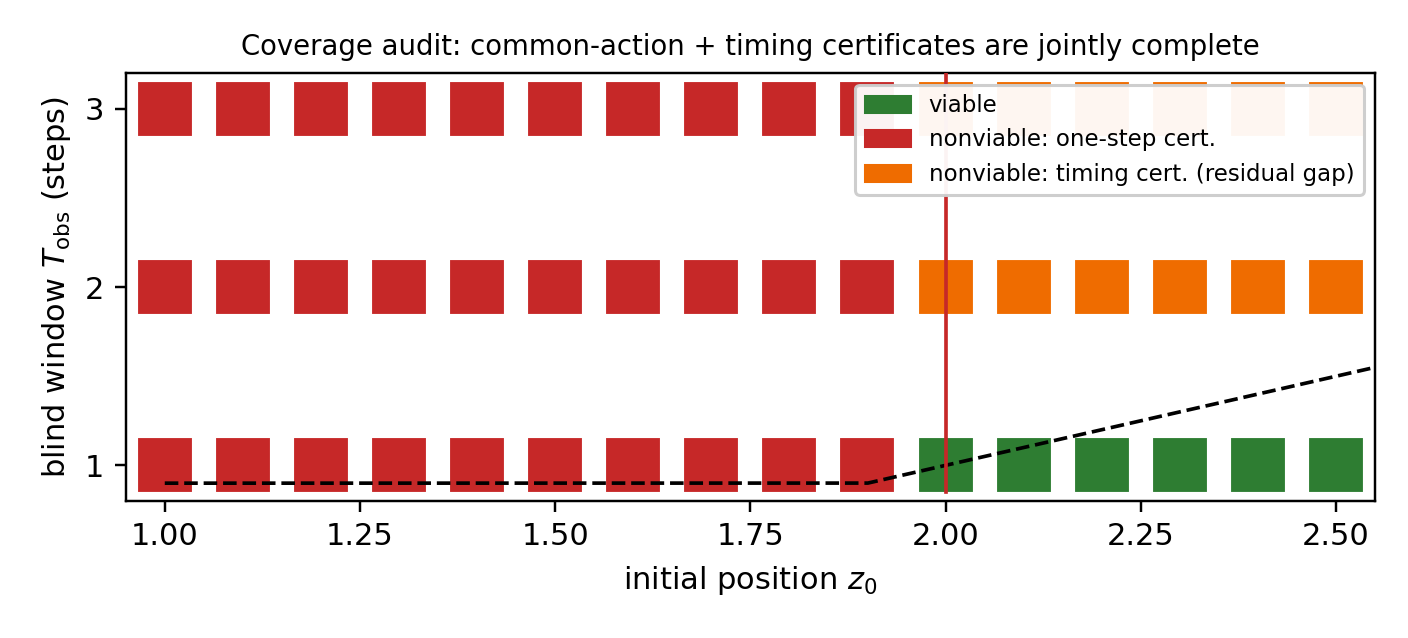
\includegraphics[width=0.82\linewidth]{figs_p2/fig_p2_coverage.png}
\caption{The coverage audit of Table~\ref{tab:coverage}: green = viable; red = nonviable, certified by the common-action certificate; orange = nonviable, certified only by the timing bound (the residual gap of Section 6.5). The dashed curve is the true boundary \(z_{0} = 1 + T_{\mathrm{obs}}\) and the solid vertical line the one-step boundary \(z_{0} = 2\).}
\label{fig:coverage}
\end{figure*}

\begin{remark}[joint completeness in the delayed class]\label{rem:coverage}
In every audited cell the true verdict is reproduced by exactly one of the two certificates: of the 42 nonviable cells, 30 are certified by the common-action certificate and the remaining 12 --- precisely those with \(z_{0} \ge 2\) and \(T_{\mathrm{obs}} > z_{0} - 1\) --- by the timing bound; none is uncovered. In this class the two certificates are jointly complete, and the Section 6.5 gap reduces to the timing cells.
\end{remark}

The audit is symbolic and one-dimensional; a multidimensional belief-space
numerical campaign is deferred to future work, and the case study makes
no claim of a general-purpose computational calculus.

\subsection{9. A Probabilistic Development: Belief-State Safety Values}\label{probabilistic-development}

The certificates of Sections 3--4 rest on set-membership semantics: the information state is a set of compatible states. This section records the stochastic counterpart --- the belief-state safety value of partially observable control --- and its obstruction certificate, connecting the calculus to the partially observable literature (\r{A}str\"om, 1965; Smallwood and Sondik, 1973).

Let \(X, A, D, Y\) be finite, with a stochastic transition \(T(x' \mid x, a)\) and an observation likelihood \(g(y \mid x, a, x')\). Augment the state space with an absorbing unsafe state \(\bot\): for \(x \in \mathcal{V}\), \(T(\bot \mid x, a) = 1 - \sum_{x' \in \mathcal{V}} T(x' \mid x, a)\), and \(T(\bot \mid \bot, a) = 1\). A belief is a distribution \(b\) over \(X \cup \{\bot\}\), updated by Bayes' rule \(\tau(b, a, y)\), with \(\mathbb{P}(y \mid b, a) = \sum_{x, x'} b(x)\, T(x' \mid x, a)\, g(y \mid x, a, x')\). The \emph{safety value} is the maximal survival probability
\[
V_{k}(b) = \max_{\pi}\; \mathbb{P}_{\pi}\bigl( x_{t} \in \mathcal{V} \text{ for } t = 0, \dots, k \;\big|\; b \bigr).
\]

\begin{theorem}[belief-state safety value]\label{thm:pomdp}
\(V_{0}(b) = b(\mathcal{V})\) (the horizon counts the current state), and for \(k \ge 0\)
\[
V_{k+1}(b) = \max_{a \in A}\; \sum_{y \in Y} \mathbb{P}(y \mid b, a)\; V_{k}\bigl(\tau(b, a, y)\bigr),
\]
with the time convention that the policy acts, observes \(y\), then acts again. The recursion is exact on every finite horizon; it is the Smallwood--Sondik belief-state value iteration specialized to the absorbing safety reward (Smallwood and Sondik, 1973).
\end{theorem}

\emph{Proof.} Standard value iteration for the belief-state Markov decision process: conditioning on the observation after the action and applying the optimal continuation gives the identity, and the absorbing state makes \(V_{k}\) the \(k\)-step survival probability (Smallwood and Sondik, 1973). \hfill\(\square\)

\begin{proposition}[chance-constrained common-action obstruction]\label{prop:chance}
Let \(b \in \Delta(\mathcal{V})\) (so \(b(\mathcal{V}) = 1\)) and write \(p(x,a) = 1 - \sum_{x' \in \mathcal{V}} T(x' \mid x, a)\). If
\[
\sum_{x \in \mathcal{V}} b(x)\, p(x,a) \;\ge\; \delta \qquad \text{for every } a \in A,
\]
then \(V_{k}(b) \le 1 - \delta\) for every \(k \ge 1\), and the chance constraint \(\mathbb{P}_{b,\pi}(x_{0}, \dots, x_{k} \in \mathcal{V}) \ge 1 - \varepsilon\) is infeasible under every policy whenever \(\varepsilon < \delta\).
\end{proposition}

\emph{Proof.} The one-step survival probability under action \(a\) is \(1 - \sum_{x} b(x)\, p(x,a) \le 1 - \delta\), so \(V_{1}(b) \le 1 - \delta\). Since \(V_{k+1} \le V_{k}\) --- more steps cannot raise the survival probability --- \(V_{k}(b) \le V_{1}(b) \le 1 - \delta\). \hfill\(\square\)

\begin{proposition}[degenerate (deterministic) limit]\label{prop:degenerate}
Let \(X, A, D, Y\) be finite, fix the deterministic maps \(x^{+} = F(x,a,d)\) and \(y = O(x,a,x^{+})\) of Section 3.1, and suppose the stochastic transition and likelihood have supports \(\{F(x,a,d) : d \in D(x)\}\) and \(\{O(x,a,x^{+}) : x^{+} \text{ reachable}\}\), converging to the corresponding Dirac measures uniformly in \((x,a)\). Then, for a belief \(b\) carried by a set \(B \subseteq \mathcal{V}\), \(V_{k}(b) \to 1\) if \(B \in \mathcal{W}_{k}\) and \(V_{k}(b) \to 0\) otherwise.
\end{proposition}

\emph{Proof.} On the finite simplex product, value iteration is continuous in \((T, g)\) uniformly in \((x,a)\). At the limit the posterior support is exactly the set-valued post-state \(\mathrm{Post}(B, a, y)\) of Section 3.1, and the recursion becomes \(V_{k+1}(B) = \max_{a} \min_{y \text{ possible}} V_{k}(\mathrm{Post}(B,a,y))\) with \(V_{0}(B) = 1\); by Theorem~\ref{thm:finite-horizon} its value is the indicator of \(B \in \mathcal{W}_{k}\). \hfill\(\square\)

Proposition~\ref{prop:degenerate} is the sense in which the chance-constrained obstruction degenerates to the common-action obstruction: at the deterministic limit \(V_{1}(b) = 1\) exactly when some action keeps every branch of the support in \(\mathcal{V}\), i.e.\ when the common safe-action set is nonempty. It is a finite-model statement; a continuous-state limit requires uniform concentration of the kernels, which is not developed here.

\subsection{10. Conclusion}\label{conclusion}

Under standard finite-dimensional regularity assumptions, viability under perfect measurement has a mature kernel, tangency, and approximation theory. Viability under incomplete observation has
long been asymmetric: the sufficiency side is carried by Veliov's
output-feedback condition and the estimation-tube programme, while the failure side has received less systematic treatment. This paper supplies the missing instrument: the obstruction calculus develops sound, computationally interpretable certificates for nonviability --- that is, sufficient conditions for nonviability, equivalently necessary conditions for viability. They do not exhaust the complement of the epistemic kernel (Section 6.5), and the paper claims no complete characterization. The mechanisms
are organized by one selector principle (Proposition~\ref{prop:selector}) --- observation-based viability
is the existence of a common recursively safe response --- and are
nested in an obstruction ladder (Proposition~\ref{prop:ladder}); in
finite systems backward belief recursion is sound and complete
(Theorem~\ref{thm:finite-horizon}), so the calculus is exact where it
can be and sound elsewhere.

With displayed proofs and explicit witnesses, the certificates identify
five mechanisms by which an observation structure can make robust
viability impossible, plus one through which a single uncorrected policy
empties the kernel: the disturbance can enforce exit in finite time
against every control; a constant observation can merge states with
incompatible admissible controls (Proposition~\ref{prop:emptiness}'s admissibility form);
the compatible states can demand incompatible actions at a single
information state; the information can arrive after the enforced exit;
and the observation fibres can cross the safe-set boundary, defeating
every exact certifier --- with the uncorrected certainty-equivalence controller as the
sixth, policy-specific, mechanism. Each certificate that admits a design
remedy identifies it: a faster indicator, a separating observation, an
observation that separates the sides of each floor instead of aggregate
certification, or the correction of a known bias. For sustainability
governance, where observation is conducted through coarse indicators at
discrete reviews, the calculus states the quantitative limits of what
monitoring can deliver --- and converts each impossibility into a design
specification. Three extensions complete the picture: the certificates are complete in the one-step and static-observation classes, with the residual dynamic gap stated as an open problem (Section 7); a calibrated case study and a coverage audit show the certificates reproducing the exact recursion verdict on a grid of delayed hidden-regime systems (Section 8); and the probabilistic belief-state lift connects the calculus to the partially observable control literature (Section 9).



\subsection{References}\label{references}
{\footnotesize

\r{A}str\"om, K.J.: Optimal control of Markov processes with incomplete state information. J. Math. Anal. Appl. \textbf{10}, 174--205 (1965)

Abaee, A.: The limits of compensatory aggregation: a formal separation of weak and strong sustainability assessment. Zenodo. https://doi.org/10.5281/zenodo.22545740 (2026).

Aubin, J.-P.: Viability Theory. Birkh\"auser, Boston (1991)

Aubin, J.-P.: Viability kernels and capture basins of sets under differential inclusions. SIAM J. Control Optim. \textbf{40}(3), 853--871 (2001)

Aubin, J.-P., Bayen, A.M., Saint-Pierre, P.: Viability Theory: New Directions, 2nd edn. Birkh\"auser, Boston (2011)

Aubin, J.-P., Catt\'e, F.: Bilateral fixed-points and algebraic properties of viability kernels and capture basins of sets. Set-Valued Anal. \textbf{10}, 379--416 (2002)

Aubin, J.-P., Frankowska, H.: Set-Valued Analysis. Birkh\"auser, Boston (1990)

B\'en\'e, C., Doyen, L., Gabay, D.: A viability analysis for a bio-economic
model. Ecol. Econ. \textbf{36}, 385--396 (2001)

Cardaliaguet, P., Quincampoix, M., Saint-Pierre, P.: Differential games
through viability theory: old and recent results. In: J\o{}rgensen, S.,
Quincampoix, M., Vincent, T.L. (eds.) Advances in Dynamic Game Theory.
Annals of the International Society of Dynamic Games, vol.~9, pp.~3--35.
Birkh\"auser, Boston (2007)

Clark, C.W.: Mathematical Bioeconomics: The Optimal Management of Renewable Resources, 2nd edn. Wiley, New York (1990)

De Lara, M., Doyen, L.: Sustainable Management of Natural Resources:
Mathematical Models and Methods. Springer, Berlin (2008)

Doyen, L., Gajardo, P.: Sustainability standards, multicriteria maximin,
and viability. Nat. Resour. Model. \textbf{33}(3), e12250 (2020)

Doyen, L., Th\'ebaud, O., B\'en\'e, C., Martinet, V., Gourguet, S., Bertignac,
M., Fifas, S., Blanchard, F.: A stochastic viability approach to
ecosystem-based fisheries management. Ecol. Econ. \textbf{75}, 32--42
(2012)

Farkas, J.: Theorie der einfachen Ungleichungen. J. Reine Angew. Math.
\textbf{124}, 1--27 (1902)

Frankowska, H.: Optimal trajectories associated with a solution of
contingent Hamilton--Jacobi equations. Appl. Math. Optim. \textbf{19},
291--311 (1989)

Gale, D.: The Theory of Linear Economic Models. McGraw-Hill, New York
(1960)

Haddad, G.: Monotone viable trajectories for functional-differential
inclusions. J. Differ. Equ. \textbf{42}, 1--24 (1981)

Hale, J.K., Verduyn Lunel, S.M.: Introduction to Functional Differential
Equations. Springer, New York (1993)

Kurzhanski, A.B., V\'alyi, I.: Ellipsoidal Calculus for Estimation and
Control. Birkh\"auser, Boston (1997)

Maghenem, M., Sanfelice, R.G.: Characterizations of safety in hybrid
inclusions via barrier functions. In: Proceedings of the 22nd ACM
International Conference on Hybrid Systems: Computation and Control
(HSCC), pp.~109--118 (2019)

Martinez-Alier, J., Munda, G., O'Neill, J.: Weak comparability of values
as a foundation for ecological economics. Ecol. Econ. \textbf{26}(3),
277--286 (1998)

Nagumo, M.: \'Uber die Lage der Integralkurven gew\'ohnlicher
Differentialgleichungen. Proc. Phys.-Math. Soc. Japan 24, 551--559
(1942)

Prajna, S., Jadbabaie, A.: Safety verification of hybrid systems using
barrier certificates. In: Alur, R., Pappas, G.J. (eds.) Hybrid Systems:
Computation and Control (HSCC 2004). LNCS, vol.~2993, pp.~477--492.
Springer, Berlin (2004)

Prajna, S., Jadbabaie, A., Pappas, G.J.: A framework for worst-case and
stochastic safety verification using barrier certificates. IEEE Trans.
Autom. Control \textbf{52}(8), 1415--1428 (2007)

Prajna, S., Rantzer, A.: On the necessity of barrier certificates. IFAC
Proc. Vol. \textbf{38}(1), 526--531 (2005)

Quincampoix, M., Veliov, V.M.: Viability with a target: theory and
applications. In: Control Theory, Multivariate Analysis and
Applications, pp.~47--63. Springer (1994)

Saint-Pierre, P.: Approximation of the viability kernel. Appl. Math.
Optim. \textbf{29}, 187--209 (1994)

Smallwood, R.D., Sondik, E.J.: The optimal control of partially
observable Markov processes over a finite horizon. Oper. Res. 21(5),
1071--1088 (1973)

Sontag, E.D.: Mathematical Control Theory: Deterministic Finite Dimensional Systems, 2nd edn. Springer, New York (1998)

Veliov, V.M.: Sufficient conditions for viability under imperfect
measurement. Set-Valued Anal. \textbf{1}, 305--317 (1993)

Witsenhausen, H.S.: A counterexample in stochastic optimum control.
SIAM J. Control \textbf{6}(1), 131--147 (1968)

}

\section*{Declarations}

\textbf{Funding.} None.\quad \textbf{Competing interests.} None.\quad \textbf{Data availability.} No data were used; all constructions are symbolic.\quad \textbf{Code availability.} No code was used or produced; all constructions are symbolic.\quad \textbf{AI declaration.} GLM (Z.ai), Qwen (Alibaba Cloud) and DeepSeek AI assisted with drafting and iterative review.

\end{document}
